%%%%%%%%%%%%%%%%%%%%%%%%%%%%%%%%%%%%%%%%%%%%%%%%%%%%%%%%%%%%%%%%%%%%%%%%%%%%%%%%
% EIBO: Certification-Grade epsilon-Indistinguishability Brackets for Open-Set
% Encrypted-Traffic Recognition
%
% Target: USENIX Security 2027, Cycle 2.
% Template: official USENIX Security 2027 LaTeX author kit (usenix.sty).
% Body limit: 13 pages. References and appendices unlimited.
%%%%%%%%%%%%%%%%%%%%%%%%%%%%%%%%%%%%%%%%%%%%%%%%%%%%%%%%%%%%%%%%%%%%%%%%%%%%%%%%

\documentclass[letterpaper,twocolumn,10pt]{article}
\usepackage{usenix}
% natbib must come after usenix.sty: usenix loads the `cite` package, and
% natbib redefines the citation commands on top of it.
\usepackage[numbers,sort&compress]{natbib}
\usepackage{amsmath}
\usepackage{mathtools}
\usepackage{amssymb}
\usepackage{amsthm}
\usepackage{booktabs}
\usepackage{graphicx}
\usepackage{multirow}
\usepackage{seqsplit}
\usepackage{cleveref}
% Keeps appendix floats from drifting past the References heading.

% cleveref must be told about the natbib-style theorem of equations/tables
\crefname{table}{Table}{Tables}
\crefname{figure}{Figure}{Figures}
\crefname{section}{Section}{Sections}
\crefname{equation}{Equation}{Equations}
\newtheorem{lemma}{Lemma}

% shorthands used throughout the paper
\newcommand{\tv}{\mathrm{TV}}
\newcommand{\epslo}{\ensuremath{\epsilon_{\mathrm{lo}}}}
\newcommand{\epshi}{\ensuremath{\epsilon_{\mathrm{hi}}}}
\newcommand{\alaw}{\ensuremath{\alpha_{\mathrm{law}}}}
% the binomial test's null rate is its own symbol: alpha is the confidence level
\newcommand{\ptest}{\ensuremath{p_{\mathrm{null}}}}
\newcommand{\abs}[1]{\left\lvert #1 \right\rvert}

\title{\Large \bf Certification-Grade $\epsilon$-Indistinguishability Brackets\\
  for Open-Set Encrypted-Traffic Recognition}

\author{Anonymous Submission}
\date{}

\begin{document}
\maketitle

\begin{abstract}
Encrypted-traffic detectors publish accuracy with no stated limit, so a
practitioner cannot say what pairwise error is impossible for a given
observation window. We measure a two-sided $\epsilon$-indistinguishability
bracket on real QUIC wire data, one certificate per service pair, whose upper
side is a finite-sample bound on the total variation distance between that
pair's prefix laws and whose lower side is a classifier-based bound at a nominal
confidence level. The certified object is pairwise: its decision-theoretic
content is the two-point bound on a test between those services, and we claim no
multi-class or open-set reduction.

At the coarsest pre-registered channel, 336 of 990 service pairs (33.9\%) admit
such a certificate, the upper side being the scarce one at the rung where the
gate is defined; because the pairs form a complete graph over 45 services they
are not independent, and a service-cluster interval gives $[26.5\%, 43.1\%]$.
Raising the alphabet resolution is associated with higher divergence and
destroys the certificate at the same time, since the confidence radius grows with
the alphabet while the threshold does not; the upper-side set falls from 340 pairs
to none four rungs finer, and the boundary has a closed form. Where the
certificate is lost, a divisibility bound keeps the large-prefix regime
non-empty under a realizability assumption. On an independent corpus the lower
side reproduces almost exactly (0.9967 against 0.9960) while the joint gate
falls to 15.75\% under that corpus's capped lower-side convention; the gap is
significant before matching but not statistically resolved at matched evidence.

We validate the bracket against real detectors: on the 340 pairs in the
informative stratum, the observed floor-violation rates of a three-model panel
(0.6--2.9\%) fall below the 5\% null rate ($p = 0.9765$ at the strongest cell;
under the $2.5\%$ null implied by the $0.975$ joint level, $p = 0.346$), so no
detector's closed-set violation rate exceeds the certified floor. The compared
quantity is a closed-set error surrogate and we scope the claim to it. The paper also reports one methods and
limits finding: the standard chain-rule estimator returns sublinear growth on a
source whose divergence is known, so it cannot adjudicate whether divergence
grows sublinearly across dependent packet positions.
\end{abstract}


\section{Introduction}
\label{sec:intro}

A traffic classifier that reports 97\% accuracy on a benchmark has told you
almost nothing about what is achievable on your network. It has not told you
whether 99\% is reachable with a longer observation window, whether 97\% is
already at the limit the channel permits, or whether the remaining 3\% is
irreducible for reasons that have nothing to do with the classifier. Detectors
in this area are evaluated by their own error rates, and an error rate is a
statement about one system rather than a statement about the problem.

What a practitioner needs is the other direction: a bound on how well
\emph{any} classifier can do, at a stated observation window, for a stated pair
of services. The ingredients for that exist, but they share a limitation that
matters here. Classical work gives feature-conditional bounds for closed-set
fingerprinting, and recent work establishes that side-channel leakage is
inevitable under explicit conditions and characterizes a rate-distortion
frontier for defense. Both are single-letter or i.i.d.-conditional: exponential
error decay requires repeated conditionally independent observations, and the
frontier is proved inside a stationary-memoryless class. Real packet prefixes
are neither independent nor stationary, and the gap between what those results
assume and what a trace provides is exactly the gap a practitioner must cross.

We call the resulting object \emph{certification-grade}: every number it reports
is tied to a stated confidence level and a stated assumption, each named rather
than borrowing strength from the other.

We measure a two-sided indistinguishability bracket on real encrypted traffic
instead, and we give each side a confidence level rather than pairing a proven
side with an unproven one. The upper side is a finite-sample bound on the total
variation distance between two services' prefix laws, with a radius whose two
terms we derive explicitly. The lower side is a classifier-based bound at a
nominal confidence level, distribution-free in the same sense. The two sides
differ in construction and in tightness, not in whether a guarantee is
available: the upper radius is fixed by the alphabet and the flow counts, while
the lower bound must hold against an adversarial choice of decision function and
is correspondingly wider. It is the upper side that an error-floor claim needs
and the upper side that in practice binds, which is a statement about this
construction rather than about what is provable.

The bracket is computable, and it is computable at a resolution that is
deliberately coarse. On the CESNET-QUICEXT-25 XS subset, at the coarsest channel
we pre-register, 336 of 990 service pairs (33.9\%) admit an interval whose upper
side is finite-sample strict and whose lower side clears the gate
(\Cref{tab:bracket}). \Cref{fig:bracket} shows the measurement end to end: raw
flow records are quantized into a prefix symbol, the symbol feeds an upper and a
lower branch that carry different certification strength, and the two branches
meet only at the gate. The certificate is not free: raising the alphabet
resolution makes the channel more informative and destroys the certificate at
the same time, because the confidence radius grows with the alphabet size while
the threshold does not. The upper-side set falls from 340 pairs at the coarsest rung
to none four rungs finer, and the joint gate admits 336 at that rung because four
pairs clear the upper side and fail the lower (\Cref{fig:horizon}). The coarse
channel is therefore not a concession to tractability but the only regime in
which a two-sided certificate exists at these prefix lengths and flow counts.

We also report a negative result that we consider part of the contribution. The
natural estimator for how divergence accumulates across dependent packet
positions is a chain-rule plug-in, and it cannot answer the question on this
data. On a synthetic source whose analytic per-position divergence is known
exactly, the estimator returns sublinear growth, deflating its estimate to
$0.6769$ of the truth on the plain arm at the longest prefix
(\Cref{fig:estimator}). The cause is measured rather than conjectured: prefix
occupancy collapses as the prefix lengthens, and a per-position smoothing bias
accumulates exactly where contexts are sparse. Two independent repairs both fail
their known-truth gate, and the repair that would work discards more than half
the data at the upper end of the range. We report this as a methods and limits
finding, not as an estimate of a growth rate, and the question is left open with
the reason stated in numbers.

\paragraph{Contributions.}
\begin{itemize}
  \item \textbf{A pairwise indistinguishability certificate on real encrypted
  traffic.} We compute a per-pair interval whose upper side is a finite-sample
  bound and whose lower side is a classifier-based bound at a nominal confidence
  level, measured over all 990 pairs at the coarsest pre-registered channel
  (\Cref{sec:design}, \Cref{sec:results/bracket}). 33.9\% of pairs satisfy the
  joint gate, and at that rung the upper side is the scarce object. The
  certified object is the pair: its content is the two-point bound on a test
  between those two services, and we make no multi-class claim.
  \item \textbf{The certificate horizon, as a function rather than a number.}
  We show that a finer alphabet resolves more and certifies less, that the
  upper-side set is empty at and beyond the fourth rung, and that the boundary has a
  closed form in resolution, sample size, and distance whose two derivation
  routes agree to zero (\Cref{sec:results/horizon}). Where the certificate is
  lost, a conditional divisibility bound keeps the large-prefix regime
  non-empty.
  \item \textbf{A methods and limits finding for the growth question.} The
  standard chain-rule estimator cannot adjudicate whether divergence grows
  sublinearly here: its bias manufactures the effect it is meant to detect, and
  the failure is robust to two independent repairs at a quantified data cost
  (\Cref{sec:results/estimator}).
  \item \textbf{Bracket validation against real detectors and an independent
  corpus.} On the informative stratum the panel's floor-violation rates fall
  below the null rate, so no detector breaches the certified floor
  (\Cref{sec:results/detector_validation}). The lower side reproduces across
  corpora; the joint gate does not, and the difference is not statistically
  resolved at matched evidence (\Cref{sec:discussion/robustness}).
  \item \textbf{A confound that blocks the obvious corroboration.} A
  heterogeneous-i.i.d.\ null, in which every flow draws its own rate and then
  emits independent bits, reproduces the first-order-Markov vote that would
  otherwise look like evidence of within-flow dependence; the vote is therefore
  not diagnostic (\Cref{sec:results/estimator}).
  \item \textbf{Two further measured quantities that bound the scope.} A second
  certified object over whole-flow rectified statistics is reported alongside the
  prefix law, and its agreement with it is cancellation rather than
  corroboration, so the two may not be ranked (\Cref{sec:discussion/objects}).
  The unknown-class mass a bracket omits is estimated as a deployment-site
  quantity rather than a universal prior (\Cref{sec:discussion/missing_mass}).
\end{itemize}

\paragraph{Novelty boundary.} To our knowledge, no prior work measures a
two-sided bracket with asymmetric guarantee strength on real encrypted traffic,
where the asymmetry is one of constant provenance and confidence-level kind
rather than provenness; \Cref{sec:related/novelty} gives it in full.

\paragraph{Scope.}
The bracket is a measurement instrument, not a vulnerability. We consume a
(direction, size) channel and no name, address, or content field, and we quantify
what including an identifier would change rather than assuming it is immaterial.
The certified fraction is a stratum statement, and we state the stratum wherever
we quote it.

\begin{figure}[t]
\centering
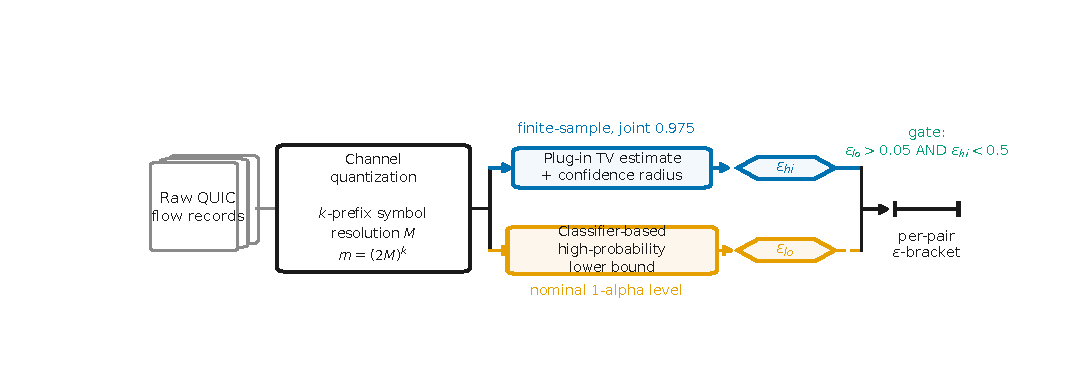
\includegraphics[width=0.86\columnwidth]{figures/paper/fig1_bracket_overview.pdf}
\caption{The EIBO measurement. Raw QUIC flow records are quantized into a
$k$-prefix symbol over a (direction, size) alphabet at resolution $M$. The
quantized symbol feeds two branches that carry different certification
strength: an upper branch combining a plug-in TV estimate with a confidence
radius, which is finite-sample, and a lower branch built from a
classifier-based high-probability lower bound whose constant is asymptotically
derived, so its level is nominal. The
branches meet at the per-pair interval, whose gate is the conjunction
$\epslo > 0.05$ and $\epshi < 0.5$.}
\label{fig:bracket}
\end{figure}


\section{Background}
\label{sec:background}

\subsection{Total variation and what a bound buys}
\label{sec:background/tv}

For two distributions $P$ and $Q$ over the same finite alphabet, the total
variation distance $\tv(P,Q)$ in \eqref{eq:tv} is, up to a factor of one half,
the smallest error probability achievable by any test that must decide which of
the two generated an observation. This is why a bound on $\tv$ is the natural
quantity for a practitioner. An upper bound on $\tv$ translates into a floor
that no classifier can go below; a lower bound translates into a statement that
the pair is genuinely separable. Neither is available from a classifier's own
accuracy, which measures one system rather than the problem.

We write the bracket as in \eqref{eq:bracket} and call each endpoint by what it
is. The upper endpoint is finite-sample and holds at the observed flow counts
with a stated confidence, under no assumption on $P$ or $Q$ beyond a finite
alphabet; the lower endpoint is a classifier-based bound at a nominal level,
distribution-free in the same sense but conditional on the fitted decision
function. Both carry a confidence level, so we report them separately and quote
the gate as a conjunction \eqref{eq:gate} rather than folding them into one
number.

\subsection{Prior information bounds on traffic analysis}
\label{sec:background/prior}

Bounding traffic-analysis performance from information-theoretic quantities,
rather than measuring it, is well established. \citet{cherubin2017bayes} gives
feature-set-conditional Bayes-error bounds for website fingerprinting, a
closed-set floor and the closest precedent for our upper side. Work on anonymity
and quantitative information flow follows the same route, from an entropy-like
quantity or a metric on distributions toward a bound on inference
\citep{serjantov2003metric,ghaderi2010anonymous,venkitasubramaniam2008eavesdroppers,venkitasubramaniam2008chaum,chatzikokolakis2007error,chatzikokolakis2008noisy}.
Our construction differs in being an explicit interval on real trace data, with
the difference between its endpoints kept visible rather than averaged away.

The most directly relevant recent results are the side-channel leakage
inevitability theorem of \citet{liu2026inevitability} and its rate-distortion
companion \citep{liu2026rate}. The former establishes that leakage is
unavoidable under explicit non-degeneracy and distinguishability conditions; the
latter characterizes an exact leakage-cost frontier. Both are single-letter in a
specific sense. The exponential error decay in the first requires conditionally
i.i.d.\ repeated observations, and the frontier in the second is proved within a
stationary-memoryless class. Packet prefixes satisfy neither condition. Our
measurement makes no such assumption and instead reports what is certifiable
about the dependent prefix law as it stands, which is why the upper side is
distribution-free, while the lower side is a classifier-based bound whose
width is set by the adversarial choice of decision function rather than by an
exponential decay rate.

\subsection{Estimating and testing total variation}
\label{sec:background/tv_est}

Turning a bound like \eqref{eq:upper} into a usable statement requires a
confidence radius for the empirical distribution, and the classical
Kolmogorov-Smirnov style constructions supply exactly that
\citep{wei2011dkwtwo,reeve2024dkwmassart}, with high-probability and two-sample
refinements that make the constant tight enough to be informative
\citep{diakonikolas2020highprob,han2015l1distribution,jiao2018l1distance}. Two
further routes are relevant. Classifier-based methods give lower bounds from a
decision function's error rate, and \citet{michel2020high} provides the adaptive
high-probability form we use for the lower side. \citet{tao2024discriminative}
relates discriminative estimation of total variation to classification risk
under a hypothesis-class assumption, which is the route we take for the
conditional large-prefix bound where the plug-in certificate is unavailable.

Open-set generalization and learnability results
\citep{fang2021learning,garov2025closer} bound the risk of a learning procedure;
ours bounds the separation available in the data, and the two are complementary
since a learnability bound says how well a detector can be trained while a
bracket says how much room there is to train into. The unknown-class mass a
bracket over observed services omits is a separate problem with its own
literature \citep{orlitsky2016optimal,eriksson2026unseen}, used for the
site-level term in \Cref{sec:discussion/missing_mass}.

\subsection{The QUIC observable}
\label{sec:background/quic}

QUIC's wire image exposes a packet-level view from which an observer recovers
packet directions, sizes, and timing, while content stays behind encryption;
\citet{kuhlewind2022rfc} documents this for operators. We use the
(direction, size) sequence of the leading packets, with prefix length and
alphabet resolution as the two parameters we pre-register and vary. Timing is
deliberately excluded, and we measure the cost of excluding the host identifier
rather than asserting it is free.


\section{Measurement Design}
\label{sec:design}

This section defines the object we measure, the channel over which it is
measured, and the two bounds that constitute the bracket. One rule governs the
design: each side of the bracket is asserted only at the strength it can carry,
and neither side borrows strength from the other.

\subsection{Problem formulation}
\label{sec:design/problem}

Let $P$ and $Q$ be the distributions of an observable random variable for two
services $a$ and $b$. Our object is the total variation distance
\begin{equation}
  \tv(P,Q) \;=\; \tfrac{1}{2}\sum_{x} \abs{P(x) - Q(x)},
  \label{eq:tv}
\end{equation}
which lower-bounds the error of any test that distinguishes $a$ from $b$: for any
measurable test $\phi$,
$\Pr[\phi \text{ errs}] \ge \tfrac{1}{2}\bigl(1 - \tv(P,Q)\bigr)$.
A bound on $\tv$ is therefore a bound on the best achievable error, and every
statement we make about distinguishability is phrased in those terms.

We report a two-sided interval
\begin{equation}
  \epslo \;\le\; \tv(P,Q) \;\le\; \epshi ,
  \label{eq:bracket}
\end{equation}
where the two endpoints come from different statistical machinery and carry
different guarantees. $\epshi$ is a finite-sample upper bound at a stated
confidence level; $\epslo$ is an asymptotic lower bound. The interval is
certified for a pair when both endpoints exist and satisfy the gate
\begin{equation}
  \epslo > 0.05 \quad\text{and}\quad \epshi < 0.5 .
  \label{eq:gate}
\end{equation}
The gate is a conjunction, and we name both of its conditions wherever we report
a count, because a bound that clears one condition and not the other is not a
certificate. \Cref{fig:bracket} shows the pipeline end to end.

\subsection{Channel definition and hygiene}
\label{sec:design/channel}

The observable is a prefix of the packet sequence, represented by the pair
(direction, size) of each packet. We quantize each axis into $M$ bins and take
the first $k$ positions, giving an alphabet of $m = (2M)^k$ symbols. The rung
ladder is $M \in \{1,2,4,8,16\}$ and $k \in \{5,10,15,30\}$. We treat $M$ as a
discrete rung rather than a continuous knob, because the interesting behavior is
at the coarse end and a continuous sweep would obscure it.

Two properties of this channel matter for interpretation. It is coarse by
construction. The exporter we use also exposes inter-packet timing, and we
exclude it; no name, address, user-agent, or TLS-extension field is consumed by
any measurement in this paper. Second, the alphabet size $m$ is the a-priori grid
size and never the realized support. This distinction is not cosmetic. A bound
that substitutes realized support for the declared alphabet can be made to look
tighter by sampling, and it is the most common way a discrete bound of this form
is quietly invalidated.

Three hygiene rules govern every evaluation. Splits are flow-disjoint and
time-disjoint; the train and test periods do not overlap and the buffer month
between them is discarded. Packet-level splitting is prohibited, so no flow is
partially represented on both sides of a split. Address fields are randomized
where the evaluation would otherwise be exposed to a shortcut, and the masking
regime is verified rather than assumed: the padding sweep reports a padding
histogram with a single zero-valued bin and 990 usable pairs at $k{=}5$ with no
services dropped. The occupancy gate is checked before any bracket is computed.
It passes on the subset used here, and we return to the scope of that pass in
\Cref{sec:discussion}.

\subsection{The upper side: finite-sample strict}
\label{sec:design/upper}

The upper side is a plug-in estimate plus a confidence radius,
\begin{equation}
  \epshi \;=\; \widehat{tv} + r_a + r_b, \qquad
  r_i \;=\; \tfrac{1}{2}\sqrt{\tfrac{m}{n_i}}
        + \tfrac{1}{2}\sqrt{\tfrac{2\ln(2/\alaw)}{n_i}},
  \label{eq:upper}
\end{equation}
where $n_i$ is the flow count available to service $i$ and $\alaw$ is the
per-law significance level. Equation~\eqref{eq:upper} is a
Dvoretzky-Kiefer-Wolfowitz type bound: it holds for any pair of distributions on
a finite alphabet, requires no smoothness, and is valid at the stated $n$. With
$\alaw = 0.025$ and a union bound over the two laws, each side of the
bracket is a joint $0.95$ statement. The left-hand column of
\Cref{tab:bracket} is computed at this setting for all 990 pairs, with a per-row
invariant check that $\epslo \le \epshi$; no violation was recorded.

The finite-sample guarantee is what makes the upper side the side to read for an
error floor. It is also, as \Cref{sec:results/horizon} shows, the side that
binds: the radius grows with $m$, so a finer alphabet tightens nothing and
eventually destroys the certificate outright.

\subsection{The lower side: asymptotic}
\label{sec:design/lower}

The lower side is a classifier-based high-probability lower bound. We choose a
decision function from a fixed class, estimate its error rate on held-out data,
and convert that rate into a lower bound on $\tv$ through the two-point
reduction; the construction follows the adaptive cutoff form of
\citet{michel2020high}. We report it as asymptotic and do not call it a
certificate, because it is not one. Its role is to cap the achievable error
floor from above: if $\epslo$ is large, no detector can do much better than the
pair's intrinsic ambiguity, and a claim that a detector has not yet reached the
information limit should be read against it.

Because the lower bound is asymptotic and the upper bound finite-sample, the two
endpoints are not symmetric in kind, and the interval in \eqref{eq:bracket}
inherits that asymmetry. We treat this as a property of the measurement rather
than a defect to be hidden. The upper side is where a practitioner looks for a
floor that cannot be beaten at the stated window; the lower side is where one
looks to confirm that a pair is genuinely separated. Neither statement is
available at the other endpoint's strength, and this extends to how we describe
cross-corpus agreement later: a joint gate over a finite-sample upper side and
an asymptotic lower side is a mixed-strength two-sided measurement, and we do
not describe it as an exact finite-sample two-sided certificate.

\subsection{Estimation procedure and its control}
\label{sec:design/estimator}

For the question of how divergence accumulates over dependent packet prefixes,
the natural estimator is a chain-rule plug-in: estimate each conditional law
$P(x_i \mid x_{<i})$ from observed prefix counts and sum the per-position
divergences. This estimator carries a $k$-dependent bias that is invisible on
real data, so it is admitted to the real data only after it first passes a
known-truth control. The control is a synthetic source whose analytic
per-position divergence is known exactly, with a second arm built on the real
occupancy profile so that the control shares the sparsity structure of the data
it is meant to license. Only an estimator that reproduces the known growth on
that control is permitted to answer the question on real traffic. We report the
outcome of that gate in \Cref{sec:results/estimator}; it did not pass, and the
consequence is the finding we report.

\subsection{The frontier as a function}
\label{sec:design/frontier}

The certificate is not a single number but a boundary. Solving
\eqref{eq:upper} for the largest $M$ at which $\epshi$ can still fall below the
gate threshold gives a closed form in the three quantities that govern it,
$M_{\max}(k, n, \tv)$. We report the frontier as a function rather than quoting
one dataset's operating point, and we give the absolute crossover sample size
only alongside the scale at which it was evaluated, because the projection scale
and the measured scale differ by more than an order of magnitude and a reader
who compares them directly will draw the wrong conclusion.

\subsection{Reproducibility boundary}
\label{sec:design/repro}

The main text carries the protocol, the channel definition, the significance
convention, the gate, and the frontier closed form. The appendix and the
released artifacts carry the per-pair ledgers, the full 20-cell resolution
table, the sample-size stratification table, and the cross-variant comparison
for the estimator study. Every quantitative claim is tied to an experiment
identifier and resolved through a content-addressed manifest; the manifest hash,
not a working copy on any machine, is the artifact of record. Artifacts are
described in the Open Science appendix.

\begin{figure}[t]
\centering
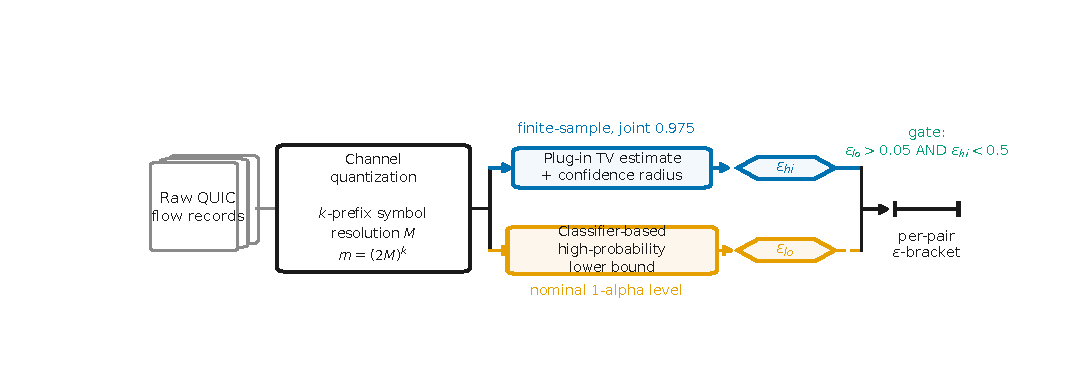
\includegraphics[width=\columnwidth]{figures/paper/fig1_bracket_overview.pdf}
\caption{The EIBO measurement. Raw QUIC flow records are quantized into a
$k$-prefix symbol over a (direction, size) alphabet at resolution $M$. The
quantized symbol feeds two branches that carry different certification
strength: an upper branch combining a plug-in TV estimate with a confidence
radius, which is finite-sample strict, and a lower branch built from a
classifier-based high-probability lower bound, which is asymptotic. The
branches meet at the per-pair interval, whose gate is the conjunction
$\epslo > 0.05$ and $\epshi < 0.5$.}
\label{fig:bracket}
\end{figure}


\section{Results}
\label{sec:results}

\subsection{Dataset and protocol}
\label{sec:results/datasets}

We measure on the \textbf{CESNET-QUICEXT-25} XS subset, a publicly released
year-long QUIC traffic corpus with extended flow attributes
\citep{cesnet2025cesnet}. From it we take the paired-design subset: captures
carrying service labels, restricted to the services and flows on which the
occupancy gate is defined.

The \textbf{990-pair denominator} comes from a flow-count threshold applied
before any bracket is computed. Of the 53 service labels present, 45 carry at
least 2{,}000 flows in the retained period, and those 45 form
$\binom{45}{2} = 990$ unordered pairs, all surviving the hygiene filters. Flow
segmentation and service selection follow a pre-registered rule
(\Cref{sec:appendix/preprocessing}), and the 2{,}000-flow threshold was fixed before the gate was
measured; the subset pass is provisional rather than a full-corpus confirmation.

The masking regime is verified rather than assumed: the padding sweep reports a
single zero-valued bin across the sampled tail slots, 990 usable pairs at
$k{=}5$, no services lost to the prefix-length filter, and identical masked and
unmasked symbol counts at every rung. A bracket over a channel that silently
included padding or address structure would be a different channel than the one
declared.

The headline $336/990$ is computed under the full-$n$ convention: every eligible
flow contributes, with no per-service cap. Both corpora were measured under both
conventions; the primary corpus's capped variant gives $335/990$ rather than
$336/990$, with pair $(21,23)$ the sole difference
($\epsilon_{\rm lo}^{\rm capped} = 0.0498$ falls below the $0.05$ gate while
$\epsilon_{\rm lo}^{\rm full\text{-}n} = 0.0588$ clears it). The
$20{,}000$-flow cap binds on 814 of the 990 primary-corpus pairs; of those,
capping raises $\epsilon_{\rm lo}$ on 38 (a 4.7\% reversal rate within the
cap-bound subset, 3.8\% of all pairs). The aggregate direction holds: 776 pairs
see $\epsilon_{\rm lo}$ decrease under capping against 38 where it increases.

\subsection{The two-sided bracket}
\label{sec:results/bracket}

\Cref{tab:bracket} (in \S A.4) is the paper's primary result. At the coarsest rung
($k{=}5$, $M{=}1$), 336 of the 990 pairs satisfy the joint gate of
\eqref{eq:gate}, a fraction of $33.9\%$. The two sides behave differently, and
that difference is the point: the upper side admits 340 pairs ($0.3434$) against
the lower side's 986 ($0.9960$), and the four-pair gap is exactly the set
passing the upper side and failing the lower. At the coarsest rung, where the joint gate is defined, the upper
side is therefore the scarce object: it is what fails relative to the lower
side, and it is what makes the certified set smaller than either side alone. At
finer resolution the lower side is not what binds: on the m-free route at
$(M{=}2, k{=}5)$ every pair clearing the upper bound also clears the lower gate,
so both counts are $127$, and on the m-free route at $(M{=}1, k{=}10)$ both are
$98$. The coarsest cell is the exception, the lower side
narrowing it by four pairs ($340\to336$). The invariant $\epslo \le \epshi$ has
zero violations on $990/990$ rows at every cell, each row's m-free upper bound
recorded. The smallest lower bound among the $127$ is $0.0755$, $0.0255$ above the
gate, against a largest measured convention effect of $0.0072$: $3.5\times$
clearance, so the identity is robust to that convention. The upper-side column of \Cref{tab:bracket} is what falls to
zero as the alphabet is refined; \Cref{sec:results/horizon} shows that the cause
is alphabet sparsity in the plug-in estimate at fine resolution rather than the
alphabet-priced radius.

The headline fraction is a stratum statement, not a property of traffic in
general: it says that 33.9\% of pairs on this corpus, at this channel, admit a
two-sided interval whose upper side is finite-sample and whose lower side clears
the gate. It does not say the remaining 66.1\% are indistinguishable: for most of
them no certificate \emph{exists} here, which \Cref{sec:results/horizon} shows is
a different and stronger statement.

\paragraph{Uncertainty on the headline.}
The 990 pairs are not independent observations: they form a complete graph over
45 services, so pairs sharing a service are correlated and a pair-level interval
would be too narrow. We therefore resample \emph{services} and report
service-level cluster-bootstrap intervals. The joint gate of $336/990 = 33.9\%$
carries a $95\%$ interval of $[26.5\%, 43.1\%]$; the upper side
$[26.8\%, 43.4\%]$; and the lower side $[99.1\%, 100\%]$. The gate interval is
wide, which is the honest statement about a corpus of 45 services; the lower
side's is tight, the same observation the gate makes, that most pairs
are separable here and the certificate is limited by the upper side.

Saturation is zero at this rung: no pair's plug-in estimate $\widehat{tv}$
reaches $0.99$, so the informative fraction is the whole corpus and the
certificate is not being purchased by discarding saturated pairs.
\Cref{tab:endpoints} in the appendix gives both endpoints' quantiles.

The same measurement on an independent corpus yields a joint gate of
$523/3321$ ($15.75\%$), an upper-side fraction of $0.1608$ and a lower-side
fraction of $0.9967$. The two results are analysed together in
\Cref{sec:discussion/robustness}, where the sample-size stratification behind the
difference, the conservative direction of its mixed-side sample sizes, and a
service-cluster bootstrap of the gap are set out.

A second certified object is computed on the same flows over whole-flow rectified
statistics rather than the $k$-prefix symbol law. At $M{=}1$ its upper side admits
292 of 990 pairs and its joint gate 289, against the prefix law's 340 and 336.
\Cref{sec:discussion/objects} shows the proximity of their informative fractions
to be cancellation, not agreement: we neither rank them nor treat either as a
check on the other.

\subsection{The certificate horizon}
\label{sec:results/horizon}

Increasing the alphabet resolution makes the channel more informative and the
certificate less available, and both effects are measured. The median $\tv$ over
pairs rises with $M$, from $0.5805$ at $M{=}1$ through $0.8833$, $0.9248$, and
$0.9462$ to $0.9673$ at $M{=}16$.

The rise is tested with paired increments rather than by comparing marginal
intervals, since the same service draws are reused at every rung and the
marginals overlap at the finer resolutions. A paired increment at a step is the
median of the paired differences
$\Delta_i = \widehat{tv}(M,\ \text{pair}_i) - \widehat{tv}(M-1,\ \text{pair}_i)$
taken over pairs, \emph{not} the difference of the two rungs' medians; the two
statistics differ because the median is not additive, and at the first step they
give $+0.2931$ (median of differences, what we report) against $+0.3028$
(difference of the two rungs' median divergences, $0.8833 - 0.5805$ from the
first line above). The paired form is the one that controls for pair identity
and carries the interval.
The paired increment excludes zero at every step: $+0.2931$ $[+0.2580,+0.3320]$ from $M{=}1$
to $2$; $+0.0438$ $[+0.0229,+0.0708]$ to $4$; $+0.0199$ $[+0.0040,+0.0429]$ to
$8$; and $+0.0131$ $[+0.0003,+0.0403]$ to $16$. The paired increment excludes
zero at every rung and shrinks by over an order of magnitude across the ladder,
though the last step is the thinnest, its lower bound
essentially on zero, so we describe the tail as still rising but flattening
rather than asserting it as firmly as the first step. One confound must be named: the increments establish that the medians rise with
significance, but do not by themselves separate genuine resolution from sparse
inflation at fixed $n$, since a finer alphabet spreads the same flows over more
symbols. The saturating column is the tell (\Cref{tab:bracket} / \Cref{fig:horizon}a). The $M{=}1$ median's marginal interval is
$[0.5079,0.6459]$.

A finer alphabet is associated with higher median divergence, but the confound
named above leaves the causal claim open. What falls is the fraction of pairs for
which an upper bound
below the gate threshold still exists: $340/990$ at $M{=}1$, $47/990$ at
$M{=}2$, $3/990$ at $M{=}4$, and zero at $M{=}8$ and $M{=}16$
(\Cref{fig:horizon}a).

We first attributed this to the radius, and that attribution was wrong.
The certified floor is $(1-\epshi)/2$ with $\epshi=\widehat{tv}+r_a+r_b$, and
$r_i$ in \eqref{eq:upper} does grow with $m=(2M)^k$. But the estimator has
already saturated before any radius is added: at $k{=}30$, $597$ of $820$ pairs
carry $\widehat{tv}\ge 0.99$ with median $0.9979$, leaving no room under the
gate threshold whatever the radius. The cause is the sparsity-driven upward bias
of $\widehat{tv}$ at fine resolution, not the alphabet-priced radius.

That distinction matters because the alphabet price is avoidable. Our
\eqref{eq:upper} bounds the $\ell_1$ norm, whose supremum runs over all $2^m$
subsets, and $\sqrt{m/n}$ is that route's cost. Bounding instead the single
population-optimal set $A^\ast=\{x:P(x)>Q(x)\}$, which depends only on the true
$P,Q$, is a two-event statement rather than a $2^m$-event one, so one-sided
Hoeffding applies directly to $P(A^\ast)$ and $Q(A^\ast)$ and no $m$ appears:
\begin{equation}
  \tv(P,Q) \;\le\; \widehat{tv}
  + \sqrt{\tfrac{\ln(2/\delta)}{2n_a}} + \sqrt{\tfrac{\ln(2/\delta)}{2n_b}} .
  \label{eq:mfree}
\end{equation}
This is a route choice, not a new theorem: both bounds are valid and certify
the \emph{same} object, an interval on $\tv(P,Q)$ for the pair, differing only in
derivation. The two-event deviation argument is the Le Cam mechanism already
used above \citep{tsybakov2009introduction}, and avoiding the alphabet term this
way is the theme of the closeness-testing line
\citep{chan2013closeness,diakonikolas2020highprob} rather than a device particular
to this paper. At our per-law level $\delta=\alaw=0.025$ the fluctuation terms
coincide exactly, $\tfrac12\sqrt{2\ln(2/\alaw)/n}=\sqrt{\ln(2/\alaw)/(2n)}$, so
the two forms differ only in $\sqrt{m/n}$ and no constant convention needs
reconciling.

Both are reported. On the same per-pair data \eqref{eq:mfree} is $2.9\times$
tighter at the coarsest rung ($M{=}1$, $k{=}5$, $n{=}2791$; per-side radius
$0.028018$ against $0.081557$), and the nominal coverage measured by the calibration design of
\Cref{tab:coverage} applies to the alphabet-priced upper side. Recomputed over the full
$(M,k)$ grid (\Cref{tab:grid}), the two bounds show two regimes rather than one. At coarse resolution the
alphabet price is what binds, and removing it buys real headroom: at the coarsest
rung ($M{=}1$) the frontier reaches $k{=}15$ with $18$ pairs certifiable where
the published bound reports zero, and the m-free route also clears $4$ pairs at
$M{=}2$ and $1$ at $M{=}4$ at that $k$. The advantage does not generalize to the finer
prefix lengths: it is present at every $M$ for $k{=}5$ and $k{=}10$, is confined
to $M{=}1,2,4$ at $k{=}15$, and is absent at $k{=}30$, so the extension is a
property of the coarse rungs rather than of the frontier as a whole. At fine resolution
sparsity reasserts the frontier regardless of the radius's form, though the
transition is gradual rather than a threshold: at $k{=}10$, saturation is
already $59\%$ at $M{=}4$ while the m-free route still certifies $10$ pairs.
When $m \gg n$ most symbol cells hold $0$ or $1$ observation, so $\widehat{tv}$
approaches $1$ mechanically: estimator bias, not a property of the traffic. A
simulation at $n{=}2791$ confirms it: at $m{=}32$ the estimator is unbiased,
while at $m{=}10^6$ its median exceeds $0.99$ even at true TV $0.2$. At
$k{=}15$, $M{=}8$, $712$ of $946$
pairs ($75\%$) already carry $\widehat{tv}\ge0.99$ with median $1.0000$, so no
bound fits under the gate whatever its construction, and the saturated fraction
climbs monotonically with $M$ at every $k$. The horizon is therefore not dissolved by dropping the alphabet
price; the price binds at the coarse end, and saturation reasserts the boundary
at the fine end, which is a boundary of the object rather than a defect of the
construction. We keep
\eqref{eq:upper} primary because the paper's counts and validations were computed
on it, and report \eqref{eq:mfree} alongside rather than substituting, so the
horizon claim rests on the comparison rather than a swap. Every cell of
\Cref{tab:grid} comes from the released per-pair ledgers, which carry all five
$M$-rungs for the same pairs at every $k$; we report the grid as measured and
interpolate nothing.

Where the plug-in certificate is lost, the large-$k$ side is not empty. A
divisibility-based lower bound, evaluated on the rung set
$k \in \{5,10,15,20,25,30\}$ (the chain-rule experiment's grid, which extends the
bracket's), is nontrivial on every pair at $k{=}15,20,25,30$, so the pivot from a
two-sided bracket to a one-sided statement is available precisely where the
certificate fails. We report this bound as conditional on its realizability
assumption and never as distribution-free.

\subsection{Detector validation}
\label{sec:results/detector_validation}

A bracket is useful only if real detectors respect it. We test this with a
pre-registered one-sided binomial comparison on the informative stratum
($\epshi < 0.5$) against the predicted floor $(1-\epshi)/2$. The stratum is populated at $k{=}5$ (340 informative, 540 secondary, 110
excluded), summing to the 990-pair denominator of \Cref{tab:bracket}. At $k{=}15$ and $k{=}30$ the stratum is empty, so those
rungs contribute no validation evidence and we say so rather than reporting a
vacuous pass.

\paragraph{Panel and protocol.}
The pre-registration was written before the first measurement, with seed 12 and
flow- and time-disjoint splits; the registration timestamp precedes the
first-measurement timestamp. Three detectors are executed and one is not.
\emph{LightGBM} is trained on the $k{=}5$ (direction, size) feature vector, with
100 boosting rounds, learning rate $0.1$, and 31 leaves, on CPU. The detector's
features are the raw direction bits and log-transformed packet sizes at each of
the $k{=}5$ prefix positions (10 dimensions), which is a strictly finer
observable than the $m{=}(2M)^k{=}32$-cell quantized alphabet on which the
certificate's radius is computed. A detector that fails to breach the certified
floor is therefore evidence about a more informative observable than the one the
bracket covers. The resolution substitution runs in the direction of an easier
test: at finer resolution both the plug-in divergence and the confidence radius
increase, which lowers the predicted floor and makes a violation easier to
observe, so a non-breach on the finer object is the stronger statement. A breach
on the finer channel would not, however, falsify the coarser certificate; this
validation is a consistency check, not a falsifiable test. The closed-set /
open-set substitution declared below runs the other way, narrowing the citable
statement to the surrogate actually measured.
\emph{Prototype} is a nearest-centre rejector in the style of prototype-radius
open-set methods \citep{qu2026sepspace}: one mean centre per service, with a
per-service acceptance radius set at a distance quantile $0.95$ of the training
points around its own centre, so a test flow is accepted when its distance to
the nearest centre falls inside that centre's radius.
\emph{RoNeTC} follows the uncertainty-quantified rejector of
\citet{wang2025reliable}: an MLP with two hidden layers of width
$\min(128, 2d)$, ReLU activations and dropout $0.20$, trained with Adam at
$10^{-3}$ for $5$ training epochs and scored by Monte-Carlo dropout sampling
($8$ passes), with rejection driven by predictive uncertainty.
A fourth detector, a Pcap-Encoder adapter, was not part of the evaluated
panel; it contributes no cells and is not counted as a pass.

\paragraph{Multiplicity and power.}
The nine cells are three detectors crossed with three holdout levels, and the
same 340 informative pairs are reused across all nine. We report each cell's
raw one-sided $p$-value against its own null and do not combine cells; the
strongest cell is $p = 0.9765$, so no correction for multiplicity could change
the verdict, and we make no family-wise claim beyond that. The binomial treats
the 340 pairs as independent draws, which they are not: they form a graph over
the same services, with a maximum pair-degree of 27, so the effective
independent sample size lies somewhere between 43 and 340 (a heuristic bound,
used conservatively). The $340$
informative pairs span $43$ of the $45$ services, under the full-$n$ convention
of \Cref{sec:results/datasets} (the other $2$ carry no informative pair). The reported
$p$-values are therefore anti-conservative. That does not affect the
no-rejection conclusion, which holds by the widest margin at the LightGBM
holdout-$0.2$ cell ($p = 0.9765$ in \Cref{tab:detectors}), but
it does mean the test has less power than the nominal figure suggests.

Power is the more serious limitation. The test's null rate is
$\ptest = 0.05$, distinct from the confidence level $\alpha$ used elsewhere, and
8 violations in 340 pairs gives $p = 0.9954$, so the design has little power
against a modest excess. The observed rates ($0.6\%$--$2.9\%$) sit below both
null rates. A threshold of $0.025$ is implied by the joint level rather than
pre-registered; under it the LightGBM holdout-$0.2$ cell, the most adverse of the
nine, gives $p = 0.346$ on its $10$ violations.
Neither rejects, so reading ``not falsified'' as evidence of a tight floor would
be a mistake: the test supports only that no gross violation is present, and
detecting a two- or three-point excess would need more informative pairs than
this channel supplies.

\Cref{tab:detectors} reports the outcome. No cell rejects the null: observed
violation rates run from $0.6\%$ to $2.9\%$ against a null rate of $5\%$, all
nine cells are below the null, so no gross violation of the floor is present. Two
qualifications travel with the table, and the first is a scope restriction
rather than a caveat. The compared quantity is a pair-level macro-average
surrogate: it is the mean of the two constituent services' \emph{closed-set}
classification-error rates, whereas the certified floor of \eqref{eq:floor} is an
\emph{open-set} error bound. The test therefore does not measure the open-set
quantity the floor bounds; the citable statement is the narrower one, that
per-pair macro-average closed-set error stays above the floor on the informative
stratum.

 A fourth detector in the intended panel is not
reported: it did not run, its cells carry no information, and it is not counted
as a pass.

\emph{A consistency check on the certificate's own object.} A logistic
regression on the same $32$-symbol one-hot representation reaches a median
balanced error of $0.366$ against a per-pair floor $(1-\epshi)/2$ (median
$0.198$), clearing its own floor on every pair ($0/990$); its implied $\tv$
(median $0.267$) is weaker than the certified lower bound (capped-convention
median $0.535$), so
the certificate is consistent with, but not tight against, the classification
risk.

\subsection{The standard estimator cannot answer the growth question}
\label{sec:results/estimator}

The remaining question is how divergence accumulates as the prefix grows: with
independent positions $D_k$ would grow linearly, and sublinear growth would mean
later packet positions add less than the first. The natural estimator is a
chain-rule plug-in over conditional laws, and we admitted it to real data only
after it passed a known-truth control whose per-position divergence is known
analytically, exactly $0.3389191441548814$, so its joint divergence grows
linearly by construction.

It did not pass, and that failure is the finding. On that analytically linear
source the estimator returned sublinear growth in both arms, including a twin
built on the real occupancy profile. Its estimate-to-truth ratio is not monotone:
it peaks slightly above $1.0$ mid-range then falls to $0.6769$ on the plain arm
and $0.8820$ on the twin at $k{=}30$, deflating divergence where the prefix is
longest (\Cref{tab:estimator} and \Cref{fig:estimator}a, both in \Cref{sec:appendix/limitations}). The mechanism is
measured, not asserted: occupancy collapses with $k$, the fraction of contexts
with fewer than five transitions rising from $0.000$ at $k{=}5$ to $0.998$ at
$k{=}30$, and the median transitions per context falling from $200{,}000$ to $1$
(\Cref{fig:estimator}b,c). A per-position smoothing bias accumulates where
contexts are sparse, biasing the fitted exponent downward.

Two independent repairs were attempted and both failed their known-truth gate.
Replacing the estimator family with a Laplace-corrected, jackknife-debiased
estimator failed on both arms. Conditioning on exposure, which restricts
attention to contexts with at least $T$ transitions, never passed at any
$T \in \{5,10,20,50,100\}$ on the plain arm, and the excluded mass needed to make
contexts well-occupied grows to $0.608$ at $k{=}30$. That last number is the
finding's teeth: the repair that would work costs more than half the data at
the upper end of the prefix range. The obstacle is structural, not a matter of
tuning, and the honest statement is that the growth question is open. A
practitioner who needs a growth-rate answer on traffic of this sparsity needs a
different measurement design, and this section says so with numbers instead of
asserting it.

One further result is reported only to show the question is non-vacuous. A
nested-model comparison of a first-order Markov law against an i.i.d. null
favored the Markov model for 45 of 45 services at every tested prefix length.
That vote is not evidence: a heterogeneous arm, in which each flow draws its own
rate and then emits symbols conditionally independently at that rate, reproduces
the same vote at $k \ge 8$. That arm is homogeneous \emph{within} a flow but not
across flows, and its symbols are not independent: two draws from one flow share
a rate, so their covariance is $\mathrm{Var}(\theta) > 0$. It is therefore an
alternative mechanism for dependence rather than a null that excludes it, and the
vote cannot separate the two explanations. The vote is consequently not
diagnostic, and we report it as a measurement artifact
rather than as support for dependence. The magnitude of the real-data statistic
does exceed what the null reproduces, so neither ``dependence is real'' nor
``heterogeneity explains it'' is the correct summary; what is established is
that the vote cannot settle the question.



\section{Discussion}
\label{sec:discussion}

\subsection{Robustness across corpora}
\label{sec:discussion/robustness}

The primary result is one corpus's number, so we repeated the measurement on an
independent one. On CESNET-QUIC22, 3,321 pairs yield an upper-side fraction of
$0.1608$ ($534/3321$), a lower-side fraction of $0.9967$ ($3310/3321$), and a
joint gate of $0.1575$ ($523/3321$) (\Cref{fig:cross_corpus}a). The lower side
reproduces across the two corpora, $0.9967$ against $0.9960$, which is not a
foregone conclusion: it is computed by a different method from the upper side and
on different data. The comparison pairs the primary corpus's full-$n$ $33.9\%$
against QUIC22's capped $15.75\%$, each figure under its own convention; capping
the primary corpus as well gives $33.8\%$, the entire difference being the single
pair $(21,23)$ crossing the lower-side threshold. The unmatched pairing keeps the
primary figure the higher of the two, conservative there but not for the claim.

The upper side does not reproduce, and two facts govern how that should be read.
The cap binds on 2{,}145 of the replication corpus's 3{,}321 pairs and lowers
$\epslo$ in aggregate there, so the reported figure is a floor and the bias is
conservative; the direction is aggregate rather than per-pair, since on the
primary corpus capping raises $\epslo$ on 38 of 990 pairs, one of them pair
35--49 (full-$n$ $0.042725$ against capped $0.043732$ in \Cref{tab:boundary}),
the construction's adaptive cutoff selection being able to raise the bound on a
subsample. Second, the gap depends on how much evidence per pair is required, and
the dependence is not monotone: on the $\epshi < 0.5$ stratum it is $-18.3$
points unmatched, $-15.5$ at a $13{,}049$-flow floor, $-9.3$ at $20{,}000$,
$-13.0$ at $40{,}000$, and $-15.4$ at $80{,}000$
(\Cref{fig:cross_corpus}b). We quote the stratum values rather than the figure's,
which plots the joint-gate fraction over a slightly different subset; the series
minimises in the middle and widens again, so ``matched evidence'' is not one
well-defined point.

Whether the gap survives at matched evidence turns on the dependence structure.
The 990 pairs form a complete graph over 45 services ($\binom{45}{2}$), as do the
$3{,}321$ replication pairs over 82 services, so pairs sharing a service are
correlated and a pair-level bootstrap is anti-conservative. Under a
service-cluster bootstrap, non-reproduction remains significant before matching
($-18.3$ points, interval $[-27.4,-10.0]$) and at the $13{,}049$-flow floor
($-15.5$, $[-28.4,-2.9]$), but the intervals at the $20{,}000$, $40{,}000$, and
$80{,}000$ floors are $[-24.2,+5.2]$, $[-30.1,+4.3]$, and $[-33.6,+2.9]$, all
including zero. The residual gap at deep matching is therefore not statistically
resolved: negative at every stratum as a point estimate, without a scale-matched
defence that survives a defensible interval. The correction widens the unmatched
gap's interval by $2.77\times$ against the lower side's $1.22\times$, so only the
gap claim is affected.

\subsection{Channel sensitivity}
\label{sec:discussion/sensitivity}

The declared channel excludes the host identifier, and we measured what
including it would change rather than asserting the exclusion is immaterial. Two
arms are compared at matched declared alphabet sizes, one appending a hash of the
destination address to the prefix symbol and one a hash of a random per-flow
identifier, on the same flows and splits. At matched resolution the two separate
before either saturates, and the radius-free difference grows with identifier
cardinality, from $0.0271$ at $B{=}2$ through $0.0885$ and $0.2271$ to $0.3136$
at $B{=}256$, then falls to $0.0150$ at $B{=}65{,}536$ where both arms saturate
and the comparison loses its content (\Cref{fig:sensitivity}, in \Cref{sec:appendix/limitations}). Below saturation
the cardinality-only arm gives no comparable separation, being two to three
orders of magnitude smaller at every rung up to $B{=}256$, so the effect tracks
identifier content and not alphabet size; in the saturated tail it reaches
$0.3829$ against the identifier arm's $0.3920$, which is why the claim is scoped
below saturation.

The scope is narrow and we keep it that way. The identifier effect is
established on the radius-free estimate $\widehat{tv}$, because the
certificate-level comparison is unavailable at every rung: one arm saturates, so
$\epshi$ cannot be compared between them, and this experiment emits no
two-sided interval at all. The citable statement is that
identifier content changes radius-free separation beyond a pure cardinality
effect. It is not that the identifier destroys the certificate or degrades the
bracket, and we make no claim of that kind.

A related check tells us something about the address field itself. The
destination address is not a function of the server name: 8,323 distinct server
names map to more than one destination address in the sampled rows. Address
structure and name structure are therefore different quantities, and an
evaluation that randomizes one is not automatically protected against the other.

\subsection{The unknown-class mass at a deployment site}
\label{sec:discussion/missing_mass}

The bracket is defined over the services present in a corpus, so it says nothing
about services absent from it, a gap we quantify as a deployment-site quantity
rather than a universal prior. Over roughly five million flows with 22,108
distinct identifiers, the estimated missing-service mass is $0.00202$, with a
nonparametric lower bound of about 18,150 unseen identifiers. It grows with
subsampling, by roughly $3.7\times$ at a 1:10 rate and $11.7\times$ at 1:100, as
expected for a well-sampled distribution and a reminder that the number belongs
to its sampling rate. We report it as a site-specific additive term and do not
fold it into the bracket.

\subsection{Two certified objects that must not be ranked}
\label{sec:discussion/objects}

Two certified objects coexist: the $k$-prefix symbol law carrying the headline
bracket, and a whole-flow rectified object on the same flows. Their informative
fractions are numerically close, but that is not a cross-check: they agree only
where each uses its own radius convention, and holding it common separates them by
hundreds of pairs. The statistics differ by about $2.7\times$ and the radius
constants by about $7.3\times$ in opposite directions, so the near-equality is
cancellation, not corroboration.

\subsection{Limitations}
\label{sec:discussion/limitations}

The certificate covers 33.9\% of service pairs on the primary corpus. The
remaining pairs are not indistinguishable; for most of them no certificate
exists at these $k$ and $n$, which \Cref{sec:results/horizon} attributes to the
plug-in estimate's upward bias at fine resolution rather than to the traffic. That should be read as an
absence of certification, not as evidence of closeness. Every number here is
measured on a subset whose occupancy pass is provisional pending full-corpus
confirmation, and on a single protocol. Three further limitations are collected
here: the lower side's level is nominal rather than exact
(\Cref{sec:design/lower}), so as a two-sided statement the interval is only as
strong as its weaker endpoint; the corpora use different lower-side conventions,
so the headline comparison is mixed-strength by construction
(\Cref{sec:discussion/robustness}); and the detector validation is a consistency
check with limited power rather than a falsifiable test
(\Cref{sec:results/detector_validation}).

\emph{Upper-side coverage, and its loss under dependence.} The upper side is a
finite-sample certificate only under i.i.d.\ flow sampling, so we calibrated that
assumption. The criterion is whether an arm's coverage falls below nominal
$0.975$, adjudicated with the \textbf{two-sided} $95\%$ Clopper--Pearson interval;
the conservative choice, since a one-sided cell is easier to pass ($0/200$
gives $0.9851$ one-sided against $0.9817$ two-sided). Under i.i.d.\ draws no informative cell loses confirmation
($0.9817$ at zero breaches in $200$). The dependent arm loses it in exactly two
cells, both at block size $B{=}64$ and the largest divergence tested: $199/200$
at $n{=}50{,}953$ ($0.9725$) and $196/200$ at $n{=}107{,}065$ ($0.9496$). We
report these as endpoints, not a trend, the ladder not
being monotone; with $200$ replicates the design has little power against a two-
or three-point shortfall.

A separate $400$-replicate ladder at $B{=}64$, true $\tv = 0.40$ and
contamination $0.1$ (a different experiment from the $200$-replicate cells
above, and the only one that locates the mechanism) shows why extra data would
not close the gap. What moves is a widening \emph{lower tail}, not a shifting
centre: misses occur when $\widehat{tv}$ falls \emph{below} the truth, the
thresholds ($0.339$--$0.374$) sitting $6$--$15\%$ under a true $\tv$ of $0.400$,
while every median $\widehat{tv}$ stays flat at or above $0.400$. Within-block
dependence thickens that tail relative to the i.i.d.\ radius, and a thinner radius
cannot exempt a tail it did not create: the point estimate plateaus at $0.9825$
across $n{=}60{,}000$, $80{,}000$ and $107{,}065$ while radii shrink
$0.0352\to0.0263$, above the $0.975$ nominal level, though the confidence
interval $[0.9643, 0.9929]$ does not resolve the direction. Past $n{=}60{,}000$
shrinkage buys nothing; if coverage were to drop below nominal at higher
dependence, a correction would need to address the estimator rather than the
sample size. The estimate also sits near the edge of what
these replicates resolve ($95\%$ interval $[0.9643, 0.9929]$ at $400$), so we
 report the direction and the plateau, not the magnitude.

\subsection{Dual-use considerations}
\label{sec:discussion/ethics}

All measurements use a public corpus collected by its operators under their own
data-handling framework. We consume flow-level metadata only, attempt no
deanonymization, and report no per-flow identifier values; the appendix sets out
the full considerations.

The bracket is simultaneously an auditing instrument and a map: it shows an
operator which pairs are near the detection limit and an adversary which are
cheap to distinguish. At the finest rung the paper demonstrates detection is
possible, so the publishable content is the existence claim rather than a new
capability, and the identifier result (\Cref{sec:discussion/sensitivity}) shows
that metadata beyond the declared channel carries separation the certificate does
not cover.





\section{Related Work}
\label{sec:related}

\subsection{Information-theoretic bounds on traffic analysis}
\label{sec:related/bounds}

The idea of bounding what traffic analysis can achieve, rather than measuring
what a particular analyzer does achieve, is well established, and the results
split by the structure they assume. \citet{cherubin2017bayes} gives
feature-set-conditional Bayes-error bounds for website fingerprinting, which is
a closed-set floor and the closest precedent for the upper side of our bracket;
its bound is conditional on the feature set the analyst chooses, so it answers
how well one can do with given features rather than how much separation the
observable carries. The anonymity and quantitative-information-flow literature
takes the complementary route, from an entropy-like quantity or a metric on
distributions toward a bound on inference
\citep{serjantov2003metric,ghaderi2010anonymous,venkitasubramaniam2008eavesdroppers,venkitasubramaniam2008chaum,chatzikokolakis2007error,chatzikokolakis2008noisy}.
Those bounds are typically evaluated on models or synthetic channels, which is
where our contribution differs: we measure an interval on captured traffic.

The nearest recent results are the leakage-inevitability theorem of
\citet{liu2026inevitability} and the rate-distortion frontier of
\citet{liu2026rate}. Both are single-letter in a precise sense that matters for
this paper. Exponential error decay in the first requires conditionally i.i.d.\
repeated observations, and the frontier in the second is proved inside a
stationary-memoryless defense class. Packet prefixes are neither conditionally
independent nor stationary, so neither result applies to the object we measure
without an assumption that the data does not satisfy. Our upper side is
distribution-free precisely so that the argument does not depend on that
assumption; the price is that the lower side is asymptotic rather than
exponential.

\subsection{Total variation estimation and lower bounds}
\label{sec:related/tv}

Turning a radius into a usable statement requires finite-sample control of the
empirical distribution, and the Kolmogorov-Smirnov family supplies it
\citep{wei2011dkwtwo,reeve2024dkwmassart} with high-probability and two-sample
refinements that tighten the constant
\citep{diakonikolas2020highprob,han2015l1distribution,jiao2018l1distance,chan2013closeness}. Two
routes give lower bounds. Classifier-based methods convert a decision function's
error rate into a separation, and \citet{michel2020high} provides the adaptive
high-probability form we use. \citet{tao2024discriminative} connects
discriminative total-variation estimation to classification risk under a
hypothesis-class assumption, which is the route the conditional large-prefix
bound follows. Our construction composes these pieces into an explicit two-sided
interval and reports the two sides separately, because the composition is where
the guarantee asymmetry becomes visible.

\subsection{Open-set recognition and its comparators for encrypted traffic}
\label{sec:related/openset}

Open-set recognition is the framing this paper's setting inherits.
\citet{scheirer2013toward} introduced the risk of novel classes at deployment,
and generalization and learnability analyses
\citep{fang2021learning,garov2025closer} characterize what can be guaranteed for
detectors that must reject unknowns. Those results bound the risk of a learning
procedure; a bracket bounds the separation present in the data. The two are
complementary, since a learnability bound says how well one can train and a
bracket says how much room there is to train into. Work on unknown-traffic
identification in the encrypted setting
\citep{hu2022opencbd,li2023facing} applies the same rejection framing to network
data and reports detector-level metrics.

Two comparators bear directly on our positioning, and we state the evidential
basis for each. \citet{shamsimukhametov2023indistinguishability} studies
indistinguishability under open TLS parameters with Encrypted ClientHello; it is
the closest protocol-privacy precedent and the work our channel declaration must
answer to, since it addresses how much of the observable survives parameter
changes while we report an interval on the observable as declared, with the
identifier's contribution measured rather than assumed away. Our knowledge of
this work is abstract-level: its publisher record and abstract were retrieved
but the full text was not, and the novelty boundary in
\Cref{sec:related/novelty} is stated accordingly. RoNeTC
\citep{wang2025reliable} represents uncertainty-aware reliable open-set
classification, and a detector of that family is one arm of our validation
panel. Against these and against prototype-radius rejection
\citep{qu2026sepspace}, the distinction we draw is not that their detectors are
weak but that their reported quantities are accuracy-style metrics with no
stated limit, whereas a bracket says what limit applies.

\subsection{Data hygiene and shortcut learning}
\label{sec:related/hygiene}

Three works together motivate the evaluation discipline this paper enforces, and
we cite them as a trio because each covers a different failure mode.
\citet{zhao2025sweet} shows that representation-learning performance in
encrypted-traffic classification can be driven by shortcut features and leakage
in the data organization. \citet{wang2026bias} provides a model-agnostic,
data-driven framework for detecting dataset-specific shortcuts and
environment-entangled correlations. \citet{wickramasinghe2025sok} systematizes
this critique across the classifier literature, which is what makes it
load-bearing rather than redundant: it establishes that the problem is a
property of the field's evaluation practice rather than of one paper's setup.
A fourth line of work turns the critique into an audit procedure rather than a
diagnosis, randomizing address fields and auditing for shortcut-induced
unreliability at evaluation time \citep{zhao2026shortcutcatcher}; the
randomization we apply is the same instrument.
Together these are why we use flow- and time-disjoint splits, prohibit
packet-level splitting, randomize address fields, and verify the masking regime
instead of assuming it. The hygiene regime in \Cref{sec:design/channel} is a
direct response to these three, and the DST\_ASN audit we report is the same
instrument applied to our own environment confound.

\subsection{Unseen-class mass and protocol context}
\label{sec:related/mass}

A bracket over observed services says nothing about services absent from the
corpus, and the unseen-species literature supplies the machinery for that gap
\citep{orlitsky2016optimal,eriksson2026unseen}, which we use for the
deployment-site term in \Cref{sec:discussion/missing_mass}. On the protocol
side, QUIC's wire image and its operational implications are documented by
\citet{kuhlewind2022rfc}, the corpus we measure on and its companion are
described by \citet{cesnet2025cesnet} and \citet{luxemburk2023cesnet}, and prior
work establishes the difficulty of analysis in this setting
\citep{smith2021website,li2023facing,jerabek2025simple,luxemburk2023encryptedquic,zhang2023applicationquic}.
Learning-based traffic analyzers are now numerous
\citep{lin2022etbert,zhao2023yatc,meng2023netgpt,cui2025trafficllm,hu2022opencbd,athanasiou2025selfdefense,dyer2012peekaboo};
our contribution is orthogonal to their architectures, since it concerns what
any of them can achieve on a declared observable rather than how one of them is
built.

\paragraph{Novelty boundary.}
\label{sec:related/novelty}
To our knowledge, no prior work measures a two-sided bracket with asymmetric
guarantee strength on real encrypted traffic. We state this as a knowledge claim
rather than a search result, and the search behind it is recorded with its own
limits: it was a motivated search whose query strings and databases were not
captured at search time, so it is not a reproducible query log, and a motivated
search can miss work phrased in different vocabulary (for example
distinguishability certificates, or tolerance intervals on distributions over
observable QoS quantities). The comparison is against the works above and the
others surveyed, each of which reports a bound on synthetic or model channels, a
closed-set error floor, or an accuracy-style detector metric, and none of which
reports a per-pair interval on captured traffic whose sides carry explicitly
different certification strength. Our closest comparator,
\citeauthor{shamsimukhametov2023indistinguishability}, is known to us at
abstract level only, so the boundary it defines is stated at that strength
rather than strengthened by assumption.


\section{Conclusion}
\label{sec:conclusion}

We turned a detector score into a statement about what no detector can achieve
on a given window, by measuring a two-sided indistinguishability bracket per
service pair on real QUIC wire data. At the coarsest pre-registered channel, 336
of 990 pairs (33.9\%) admit an interval whose upper side is finite-sample and
whose lower side is a classifier-based bound at a nominal level. The horizon is
short and its failure arithmetical rather than a property of the traffic: the
radius grows with the alphabet while the threshold does not, so the upper-side
set falls from 340 pairs at $M{=}1$ to none at $M{=}8$. Where it is lost, a
divisibility bound keeps the large-$k$ regime non-empty, and the missing-service
mass bounds what a bracket over observed services can claim.

Three directions follow: full-corpus confirmation of the occupancy pass, a
design clearing a known-truth gate while retaining the data, and other protocols
and channels, the frontier being a function of resolution, sample size, and
distance.


\appendix

\clearpage
\section*{Ethical Considerations}
\addcontentsline{toc}{section}{Ethical Considerations}

All measurements in this paper are computed on a public research corpus of
backbone traffic collected and released by its operators under their own ethics
and data-handling framework. We consume flow-level metadata only. We do not
attempt to identify users, reconstruct content, or deanonymize any flow, and we
report no per-flow identifier values. The identifier analysis in the channel
sensitivity study compares a hashed destination address against a random
per-flow identifier at matched declared resolution and reports only an aggregate
separation statistic.

The result is a defensive and auditing instrument. A certified lower bound on
the error floor tells an operator what pairwise detection performance cannot be
improved past at a stated observation window, which is the information needed to
judge whether a reported detection gain is close to the limit the channel
supports. We see no path by which the published bracket enables an attack that is
not already available to anyone with the same observable channel.

The identifier is a hash over a destination address. Hashing is not
anonymization where the address space is enumerable: a salt rotated per
measurement window would prevent cross-window linkage but is not part of the
current dataset's collection protocol.

\clearpage
\section*{Open Science}
\addcontentsline{toc}{section}{Open Science}


This appendix lists the artifacts needed to evaluate the paper's core
contributions and how the review committee can reach each one.

The artifacts this paper depends on (the complete per-pair ledgers, the
calibration and estimator payloads, and the figure generators) are carried in
the supplementary-material archive \texttt{supplementary.tar.gz}, included with
this submission and delivered through the submission system's artifact
materials; its top-level \texttt{README.md} is the entry point. The call for
papers recommends an anonymous link at submission, which we have not supplied,
and reserves a stable public link for the camera-ready version; submission-system
delivery, which the call contemplates for artifacts it treats with the same
confidentiality as the manuscript, is the access path for review. The artifacts
must be public for acceptance, and they are our own per-pair statistics over a
publicly released corpus, so that condition is met.

Every claim in this paper can be checked from the submitted bytes, without
contacting the authors: the per-pair ledgers carry the columns the bounds are
computed from, so the reported numbers are recomputable from the archive with
standard tooling. As a factual matter about the files
themselves, none of the recognized grounds for withholding artifacts applies
here: there is no licensing restriction, no harm to study subjects, and no NDA
or legal constraint on them. The artifacts are per-pair statistics over a
publicly released corpus, derived from the same channel the paper declares and
carrying nothing beyond it, so publishing them adds no capability to what
\Cref{sec:discussion/ethics} already treats as a dual-use measurement: any
reader of the paper can recompute them from the corpus.

\textbf{Worked provenance example.}
Every quantitative claim resolves through an experiment identifier to a manifest
entry carrying a \texttt{content\_sha256} over the artifact's bytes. The three
real entries below were each verified against the file's own bytes; the hashes
are the full 64 hexadecimal characters, broken across lines so they do not
stretch the spacing:
\begin{itemize}
  \item the per-pair bracket table behind \Cref{tab:bracket} is registered as
  \texttt{art\_20260913\_e5ebac} (the artifact
  \texttt{q1\_lower\_side\_full\_n.json}, 990 rows), with
  \texttt{\seqsplit{9fe81e271a386335a9526563ca03631bcdf832fa5d66d3861b2e22ec079256f5}};
  \item the headline gate count is \texttt{art\_20260914\_443901}
  (\texttt{x1\_headline\_table.json}), with
  \texttt{\seqsplit{c9f840a94644687e50e672f6cdd3c65fd0469a9045ca55d1881d11a8afd41c9c}};
  \item the uncertainty intervals are \texttt{art\_20260915\_27333a}
  (\texttt{ci\_main\_table.json}), with
  \texttt{\seqsplit{2d87922190e21f06fbd7e47ebe62f22f494c45252d84578c3ff9f888176b2c86}}.
\end{itemize}

\textbf{What ``pre-registered'' means here.}
Four commitments, each fixed before the measurement it governs: the coarsest
channel ($k{=}5$, $M{=}1$) before the gate was measured; the $0.5$ upper
threshold as the informative-stratum criterion for the detector validation, a
later timepoint and a different role from the gate itself, whose $0.05$ lower
threshold was not pre-registered
(\eqref{eq:gate}); the one-sided binomial test with its null rate of
$0.05$ and its nine cells before that test ran; and the split policy (flow- and
time-disjoint, packet-level splitting prohibited) before any evaluation. The
ordering is checkable against the artifacts themselves: the detector panel's
registration is timestamped
\nolinkurl{2026-09-14T09:35:32Z}, its first measurement
\nolinkurl{2026-09-14T09:36:33Z}, one minute later, in the same artifact that
carries both fields alongside a boolean asserting the registration preceded the
measurement. That ordering, not the word itself, is the claim.

\textbf{Released artifacts.}
\begin{description}
  \item[Measurement code.] The statcore module implementing the upper-side
  bound (\texttt{tv\_upper\_bound}) and the classifier-based lower bound
  (\texttt{tv\_lower\_bound}), together with the channel packer that maps a
  (direction, size) prefix into a symbol index for a given $M$ and $k$.
  \item[Per-pair ledgers.] The 990-row per-pair bracket table at $k{=}5$,
  $M{=}1$, carrying the upper-side bound, the lower-side bound, the saturation
  flag, and the per-side flow counts. This is the artifact behind
  \Cref{tab:bracket} and \Cref{tab:boundary}.
  \item[Detector-validation payload.] The per-pair join for the nine-cell
  containment test, the stratum assignment (340 informative, 540 secondary,
  110 excluded), the pre-registered one-sided binomial results in
  \Cref{tab:detectors}, and the trained-detector configurations.
  \item[Estimator study artifacts.] The chain-rule control on a known-truth
  source, both arms (plain and real-occupancy), and the two repair attempts
  with their known-truth gates.
  \item[Cross-corpus and sensitivity artifacts.] The independent-corpus bracket
  with its stratification table, and the channel-sensitivity dose-response.
  \item[LP artifact.] The LP-optimal weighting construction behind the
  comparison floor cited in \Cref{sec:design/problem}, with its derivation, the
  equal-weight recovery of the uniform bound, and the 200-configuration validity
  check. Registered as \texttt{art\_20260918\_fd1598} with content hash
  \texttt{\seqsplit{9d16e6ad93299c5ae3b9816f851b9830fd3a1dbb6db20e6ec442026c8884f644}}.
  \item[Constructions comparison.] The four lower-bound constructions on the
  shared per-pair input (the uniform form, the LP-weighted aggregation, the
  mixture bound and the exclude-$U$ variant), with the weights and inputs each
  consumes. Registered as \texttt{art\_20260918\_f27ba9} with content hash
  \texttt{\seqsplit{0ace3222da0fad188b9382dcbf97121c5513344db6f098672d29022e3cbe003b}}.
  \item[Joint-coverage reaggregation.] The headline floors: the uniform
  open-set error floor $0.197$ at the simultaneous level $0.95$ (Bonferroni over
  the $990$ pairs, $\alpha_{\mathrm{pair}} = 0.05/990$), the matched $M{=}45$
  floor $0.206$, the $M{=}46$ gap $0.63$, and the LP-weighted floor $0.375$,
  with the falsifier result ($984/990$ pairs non-vacuous, $6$ vacuous, zero
  $\epsilon_{\mathrm{lo}} > \epsilon_{\mathrm{hi}}$ violations). Registered as
  \texttt{art\_20260922\_f7853e} with content hash
  \texttt{\seqsplit{c05735901f4bb714c55446ee324afe354716bc0a8cd4de5df4120aae042fc218}}.
  \item[Same-channel validation.] The balanced-accuracy risk interval for the
  same-channel check in \Cref{sec:results/detector_validation}. Each pair's
  balanced error is compared against \emph{that pair's own} certified error floor
  $(1-\epsilon_{\mathrm{hi}})/2$, a per-pair quantity (median $0.198$, range
  $0$--$0.467$), not a single threshold held against all $990$: the
  zero-violation result ($0/990$) is that per-pair comparison. Registered as
  \texttt{art\_20260922\_764458} with content hash
  \texttt{\seqsplit{06c0e766f4a47280e4245ef41f72f89ade3fc6337be76a8e196074732de1e40d}}.
  \item[Upper-side coverage calibration.] The i.i.d.\ control arm and the
  dependent-contamination arm behind \Cref{tab:coverage} and the coverage
  statement in \Cref{sec:discussion/limitations}:
  \begin{itemize}
    \item \texttt{art\_20260918\_a408c2}
    (\texttt{coverage\_calibration\_v2.json}):
    \texttt{\seqsplit{b4e7f8b0755a09561736ab7bfc39318980548a0ae0cfda7243e9de48a5b399dc}}
    \item \texttt{art\_20260918\_17c1b0}
    (\texttt{coverage\_calibration\_ladder.json}):
    \texttt{\seqsplit{86bd86a27a6efe8edacfbe5cafd2b38c5b4724e5f95de8f9afa5355e3c43d29a}}
    \item companion write-ups \texttt{art\_20260918\_4b3dc7}
    (\texttt{coverage\_calibration\_v2.md}):
    {\raggedright\texttt{\seqsplit{7cb28ef9022730d21b99545fb39126dcd7c957fd9cd873333bca244e28273e08}}\par}
    and \texttt{art\_20260918\_9821af}
    (\texttt{coverage\_calibration\_ladder.md}):
    {\raggedright\texttt{\seqsplit{bf82aa240795ebdbab1cdd6170c86552daa20433a6a363103be7c7e9b88bb55f}}\par}
  \end{itemize}
  \item[Analysis loads.] The four further analyses this paper adds,
  each registered with its own content hash:
  \begin{itemize}
    \item the $5000$-replicate skewness follow-up behind \Cref{sec:appendix/track5}:
    \texttt{art\_20260920\_0e4cdb} (\texttt{track5\_skewness\_n5000.json}):
    \texttt{\seqsplit{6558da3814befb13c9d86105b973b2f5e528d9c921fd125fdd800492db329ee9}}
    \item the $400$-replicate dependence ladder behind the coverage statement in
    \Cref{sec:discussion/limitations}:
    \texttt{art\_20260918\_17c1b0} (\texttt{coverage\_calibration\_ladder.json}),
    \texttt{\seqsplit{86bd86a27a6efe8edacfbe5cafd2b38c5b4724e5f95de8f9afa5355e3c43d29a}}
    \item the full $(M,k)$ grid behind \Cref{tab:grid}:
    \texttt{art\_20260918\_a73525} (\texttt{eth\_full\_mk\_grid.json}):
    \texttt{\seqsplit{522e25ff05b7ef84fe49bdc69ea6a2bd8fc50e56a7d26c7952c3f726adb89d7f}}
    \item the threshold-sensitivity sweep behind \Cref{tab:thresholds}:
    \texttt{art\_20260918\_b5a5cd} (\texttt{eth\_T2\_T3\_results.json}):
    \texttt{\seqsplit{cee50b40b7913279144c537cc632610a28c352606c0994bda5b2e62d72bc2d17}}
  \end{itemize}
  \item[Three dependence-aware radii.] The block bootstrap, cluster-robust
  sandwich and leave-one-block-out arms of \Cref{sec:appendix/track5}, one
  artifact each:
  \texttt{art\_20260919\_17d7d3} (\texttt{track5\_armA\_block\_bootstrap.json}),
  \texttt{\seqsplit{b7bd97063a694c80d35147e1ada07a00abb573f01f1d142848936e14e62a32c8}};
  \texttt{art\_20260919\_b84113} (\texttt{track5\_armB\_sandwich.json}),
  \texttt{\seqsplit{741b321095e0aab0e7ca3a3a62f7412757a33588b5eb37caeb5ab83e4a221965}};
  \texttt{art\_20260919\_fc043c} (\texttt{track5\_armC\_lobo.json}),
  \texttt{\seqsplit{775ceede475a2f19f09ef398afe29632b02a4d8495b77270022716c013923c41}}.
  \item[Figure generators.] Scripts rebuilding every figure from its artifact,
  plus the provenance map of each series' source file and hash.
\end{description}

\textbf{Content-addressed chain of record.}
The artifacts cited in this paper are content-addressed: each carries a
\texttt{content\_sha256} over its own bytes, and that hash, rather than any
working copy, is the artifact of record. A nested-field citation is recorded in
the paper's provenance crosswalk so a reviewer can follow the number to its
source without tooling. The manifest also holds display entries that no claim in
this paper cites; those are registered for completeness and are not
content-addressed, since only the cited chain needs to be.

\textbf{Data.}
The primary corpus is publicly released by its operators and requires no
credential to obtain; the independent replication corpus is likewise public. We
redistribute neither, and instead document the acquisition steps and the
preprocessing applied to produce the flow-level tables used here.

\clearpage
\section*{Appendix: Supplementary Material}
\addcontentsline{toc}{section}{Supplementary Material}

\setcounter{subsection}{0}
\renewcommand{\thesubsection}{A.\arabic{subsection}}

\subsection{Per-Pair Ledger and Boundary Pairs}

The headline result rests on a 990-row per-pair ledger at $k{=}5$, $M{=}1$,
carrying for each pair the upper-side bound, the lower-side bound at full $n$,
the per-side flow counts, and the saturation flag. Recomputing the upper-side
condition row-by-row from that ledger reproduces the 340-pair count and the
336-pair joint gate, and the four pairs that separate them are listed in
\Cref{tab:boundary}. We report them because they are the only rows whose verdict
depends on the lower side at this rung; every other certified pair clears both
conditions by a margin.

\begin{table}[!htbp]
\centering
\caption{The four boundary pairs at $k{=}5$, $M{=}1$: each passes the upper side ($\epshi < 0.5$) and fails the lower ($\epslo \le 0.05$). These are exactly the pairs separating the 340-pair upper-side count from the 336-pair joint gate. Per-side flow counts are given because the lower side is computed at full $n$ with the 20{,}000-flow cap removed. Pair (21,23), which is not among them, is the sole pair whose verdict changes between the capped and full-$n$ conventions (\Cref{sec:results/datasets}).}
\label{tab:boundary}
\begin{tabular}{lrrrr}
\toprule
pair & $n_a$ & $n_b$ & $\epslo$ & $\epslo$ (capped) \\
\midrule
39--44 & 4624 & 5741 & 0.015071 & 0.015071 \\
11--51 & 13049 & 1399495 & 0.022607 & 0.012230 \\
27--29 & 137553 & 11462 & 0.028705 & 0.026651 \\
35--49 & 159842 & 2791 & 0.042725 & 0.043732 \\
\bottomrule
\end{tabular}
\end{table}

\begin{figure}[t]
\centering
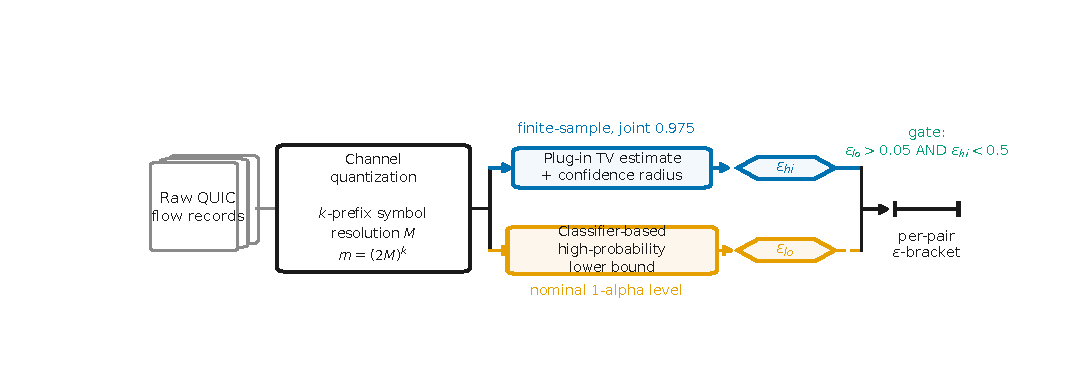
\includegraphics[width=0.86\columnwidth]{figures/paper/fig1_bracket_overview.pdf}
\caption{The measurement pipeline. Cited from \Cref{sec:intro} and
\Cref{sec:design/problem}. Raw QUIC flow records are quantized into a
$k$-prefix symbol over a (direction, size) alphabet at resolution $M$. The
quantized symbol feeds two branches that carry different certification
strength: an upper branch combining a plug-in TV estimate with a confidence
radius, which is finite-sample, and a lower branch built from a
classifier-based high-probability lower bound whose constant is asymptotically
derived, so its level is nominal. The
branches meet at the per-pair interval, whose gate is the conjunction
$\epslo > 0.05$ and $\epshi < 0.5$.}
\label{fig:bracket}
\end{figure}

\label{sec:appendix/context}
\label{sec:appendix/endpoints}

Table~\ref{tab:endpoints} gives the distributional summary of the bracket
endpoints.

\begin{table}[!htbp]
\centering
\small
\caption{Both endpoints across all 990 pairs at $k{=}5$, $M{=}1$, with width
defined as $\epshi-\epslo$. The $\epslo$ column is the \emph{uncapped}
convention (full per-service flow counts), the paper's declared convention
(\Cref{sec:results/datasets}); the capped run's median is $0.535$. The lower
bound's median sits ten times above the gate, which is what "the lower side
saturates" means quantitatively, and no bracket has negative width.}
\label{tab:endpoints}
\begin{tabular}{lrrrrr}
\toprule
 & min & p25 & median & p75 & max \\
\midrule
$\epslo$ & 0.0151 & 0.3411 & 0.5548 & 0.6990 & 0.9729 \\
width & 0.0139 & 0.0428 & 0.0784 & 0.1119 & 0.2214 \\
\bottomrule
\end{tabular}
\end{table}


\subsection{Protocol Context and Unknown-Class Machinery}

A bracket over observed services says nothing about services that are absent
from the corpus, and the unseen-species literature supplies the machinery for
that gap \citep{orlitsky2016optimal,eriksson2026unseen}, which we use for the
deployment-site missing-service-mass term in \Cref{sec:discussion/missing_mass}.

On the protocol side, QUIC's wire image and its operational implications are
documented by \citet{kuhlewind2022rfc}; the corpus we measure on is released with
its companion dataset \citep{cesnet2025cesnet,luxemburk2023cesnet}, and its
deployment has since been measured passively at scale \citep{mucke2025waiting};
and classifiers are now applied to it across a range of architectures
\citep{luxemburk2023encryptedquic,zhang2023applicationquic,lin2022etbert,zhao2023yatc,meng2023netgpt,cui2025trafficllm,hu2022opencbd,smith2021website,li2023facing,jerabek2025simple}.
Our contribution is orthogonal to those architectures, since it concerns what any
of them can achieve on a declared observable rather than how one of them is
built.

\subsection{Preprocessing and Service Selection}
\label{sec:appendix/preprocessing}

Flows follow the corpus's own five-tuple and idle-timeout convention, with no
resegmentation of our own. From each flow we read the leading packet sequence and
reduce it to the (direction, size) prefix the channel declares; no payload is
parsed, and the acquisition steps that turn a capture into the flow-level tables
used here are recorded in the released notes.

The service-eligibility rule is pre-registered rather than tuned. The
2{,}000-flow threshold was fixed before the gate was measured, so that one rule
governs every rung of the ladder. It replaces an earlier 53-service /
1{,}378-pair selection that used a lower 617-flow minimum: two selection rules
on one capture would make the resulting artifacts mutually non-citable, which is
why the stricter rule was adopted. Masking is likewise verified rather than
assumed, as \Cref{sec:results/datasets} reports.

\subsection{The Two-Sided Bracket by Rung}
\label{sec:appendix/bracket_table}

This table reports, for each resolution $M$ and prefix length $k$, the number of
pairs whose upper side alone clears the gate, that count as a fraction of the
pairs available at that $(M,k)$, the saturated fraction, and the joint-gate count
where both sides were evaluated. It prints the figure behind
\Cref{sec:results/bracket} in full.

\begin{table}[t]
\centering
\small
\caption{The two-sided bracket on the primary corpus by resolution $M$ and prefix length $k$ (this appendix, \Cref{sec:appendix/bracket_table}). \emph{Upper} is the count and fraction of pairs whose upper side alone satisfies $\epshi < 0.5$; \emph{sat.} is the fraction with $\widehat{tv} \geq 0.99$. The joint gate is reported where both sides were evaluated, at the cells
named in \Cref{sec:results/bracket}; rows carrying only the upper side are marked as such, and zero cells are listed rather than omitted. Counts here carry no uncertainty; service-cluster bootstrap intervals for the headline figures are in \Cref{sec:results/bracket}.}
\label{tab:bracket}
\begin{tabular}{rr rr rr r}
\toprule
$M$ & $k$ & pairs & upper & upper frac. & sat. & joint \\
\midrule
1 & 5 & 990 & 340 & 0.3434 & 0.0000 & 336 \\
2 & 5 & 990 & 47 & 0.0475 & 0.1051 & \textendash \\
4 & 5 & 990 & 3 & 0.0030 & 0.2394 & \textendash \\
8 & 5 & 990 & 0 & 0.0000 & 0.3364 & \textendash \\
16 & 5 & 990 & 0 & 0.0000 & 0.3909 & \textendash \\
\midrule
1 & 10 & 990 & 28 & 0.0283 & 0.0061 & \textendash \\
2 & 10 & 990 & 0 & 0.0000 & 0.2909 & \textendash \\
4 & 10 & 990 & 0 & 0.0000 & 0.5929 & \textendash \\
8 & 10 & 990 & 0 & 0.0000 & 0.6384 & \textendash \\
16 & 10 & 990 & 0 & 0.0000 & 0.6889 & \textendash \\
\midrule
1 & 15 & 946 & 0 & 0.0000 & 0.0391 & \textendash \\
2 & 15 & 946 & 0 & 0.0000 & 0.5761 & \textendash \\
4 & 15 & 946 & 0 & 0.0000 & 0.6966 & \textendash \\
8 & 15 & 946 & 0 & 0.0000 & 0.7526 & \textendash \\
16 & 15 & 946 & 0 & 0.0000 & 0.8076 & \textendash \\
\midrule
1 & 30 & 820 & 0 & 0.0000 & 0.7280 & \textendash \\
2 & 30 & 820 & 0 & 0.0000 & 0.8500 & \textendash \\
4 & 30 & 820 & 0 & 0.0000 & 0.9195 & \textendash \\
8 & 30 & 820 & 0 & 0.0000 & 0.9561 & \textendash \\
16 & 30 & 820 & 0 & 0.0000 & 0.9720 & \textendash \\
\bottomrule
\end{tabular}
\end{table}

\subsection{Supporting Detail for the Limitations}
\label{sec:appendix/limitations}

\begin{figure*}[t]
\centering
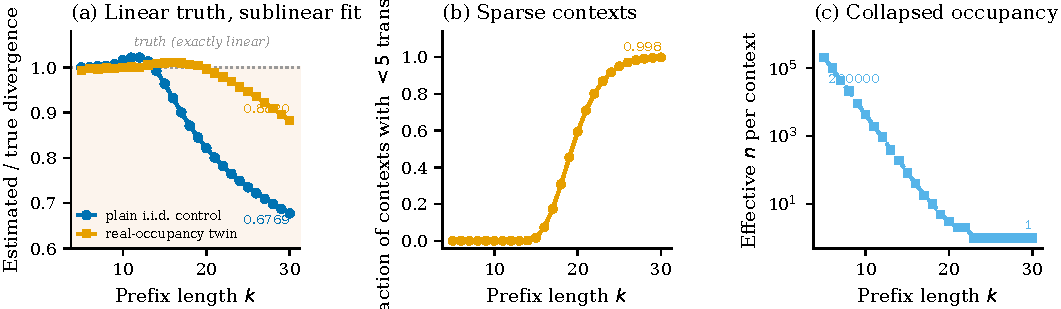
\includegraphics[width=0.64\textwidth]{figures/paper/fig3_estimator_control.pdf}
\caption{The estimator limit. (a) Estimated-to-true divergence on a source whose
analytic per-position divergence is known, for the plain-i.i.d.\ control and the
real-occupancy twin: both peak near $1.0$ then fall to $0.6769$ and $0.8820$ at
$k{=}30$. (b) Fraction of contexts with fewer than five transitions, rising to
$0.998$. (c) Median context count, falling from $200{,}000$ to $1$. The estimator
deflates divergence exactly where contexts are sparse.}
\label{fig:estimator}
\end{figure*}

\begin{figure*}[t]
\centering
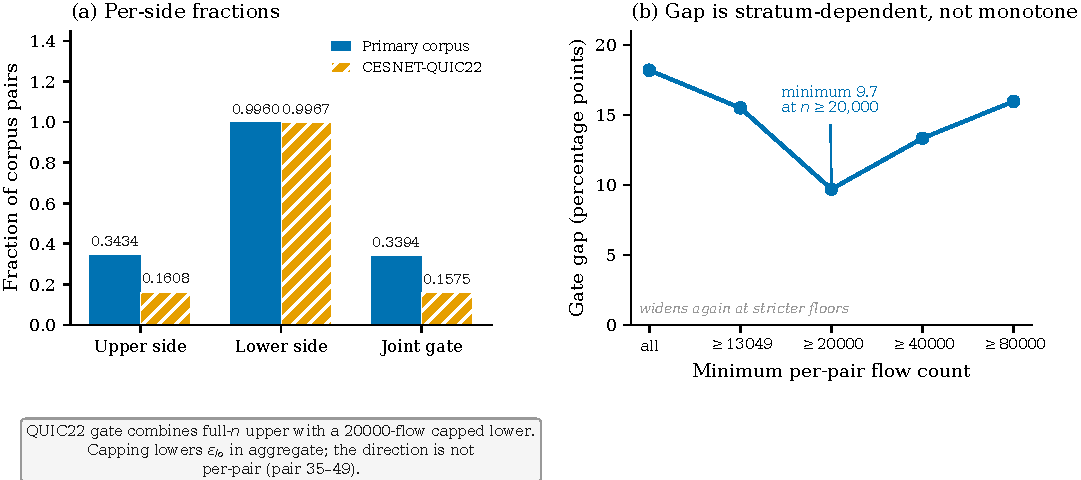
\includegraphics[width=0.62\textwidth]{figures/paper/fig4_cross_corpus.pdf}
\caption{Robustness across corpora. (a) Per-side fractions on the primary corpus
and on CESNET-QUIC22: the lower side reproduces almost exactly ($0.9960$ against
$0.9967$) while the upper side and joint gate differ. The QUIC22 joint gate
combines a full-$n$ upper side with a capped lower side (hatched), so it is a
mixed-strength measurement rather than an exact finite-sample certificate. (b)
The gate gap by minimum per-pair flow count: largest unmatched, at a minimum at
$20{,}000$, then widening again, so the series is not monotone and ``matched
evidence'' is not one point. Under a service-cluster bootstrap the unmatched gap
excludes zero while the deeper strata do not.}
\label{fig:cross_corpus}
\end{figure*}

\emph{The certificate horizon.} The rung-ladder result behind \Cref{sec:results/horizon} is shown in \Cref{fig:horizon}.

\begin{figure*}[t]
\centering
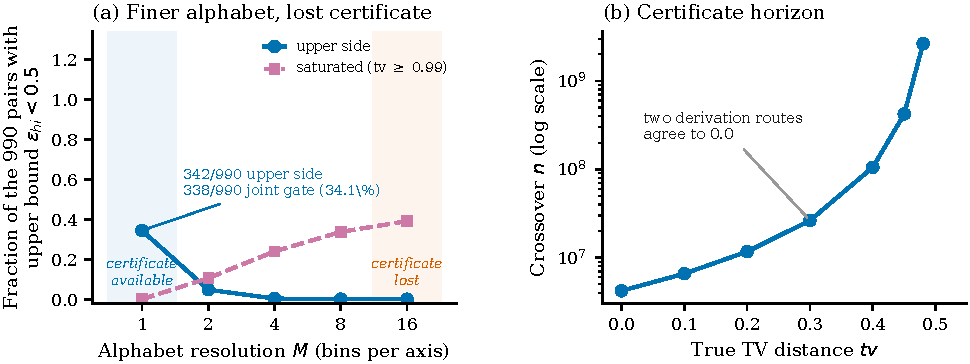
\includegraphics[width=0.64\textwidth]{figures/paper/fig2_certificate_horizon.pdf}
\caption{The certificate horizon. (a) The fraction of the 990 pairs whose upper
side alone satisfies $\epshi < 0.5$ against resolution $M$ at $k{=}5$: it falls
from $340/990 = 0.3434$ at $M{=}1$ to zero at $M{=}8$, while the saturated
fraction rises from $0.000$ to $0.391$. The annotation gives both the upper-side
count and the joint gate ($336/990$), which exists at $M{=}1$ only. (b) The
crossover sample size at which the $M{=}8$ certificate ceases to exist, against
true TV distance; two derivation routes agree to zero absolute difference.}
\label{fig:horizon}
\end{figure*}

Three limitations are stated in one sentence each in the body; the supporting
detail is collected here.

\emph{The frontier's closed form, and its limit.} The closed form is \eqref{eq:mmax},
derived and displayed once in \Cref{sec:appendix/thresholds}; what belongs here
is its limit. It is the certifiability criterion $\widehat{tv} +
\text{radius} < 0.5$, not the radius alone, which is necessary but not
sufficient; the two coincide only at $\widehat{tv} = 0$. We report the crossover
only alongside the scale it was evaluated at, since the projection scale and the
measured scale differ by more than an order of magnitude.

The closed form is derived from \eqref{eq:upper}, so it inherits that bound's
$\sqrt{m/n}$ term and describes the frontier \emph{of that route}, not of the
problem. The same criterion written with \eqref{eq:mfree} has no $m$ in it at
all: $0.5 - \widehat{tv} - \sqrt{\ln(2/\delta)/2}\,
\bigl(n_a^{-1/2}+n_b^{-1/2}\bigr) > 0$, which no alphabet size can satisfy once
$\widehat{tv}$ saturates, however large $k$ grows. The $1/k$ exponent is
therefore a property of the alphabet-priced route rather than a fact about the
channel, and the operative constraint at fine resolution is alphabet sparsity in
the plug-in estimate of $\widehat{tv}$ (\Cref{sec:results/horizon}), which
neither form can repair.

\emph{Lower-side status.} The lower side's constant is asymptotically derived
and a conservative finite value is substituted only in the degenerate regime
where the effective alphabet is too small for the asymptotic expression to be
defined (\Cref{sec:design/lower}). The $1-\alpha$ label is therefore what the
construction reports rather than a finite-sample guarantee, and the large-$k$
divisibility bound is separately conditional on a realizability assumption:
useful exactly where the plug-in certificate is lost, but not distribution-free.

\emph{Convention dependence.} The corpora use different lower-side conventions,
the primary at full $n$ and the replication at a $20{,}000$-flow cap. The cap's
effect is aggregate rather than per-pair: it lowers $\epslo$ on 776 of the 990
primary-corpus pairs and raises it on 38, which is why we report an aggregate
direction and do not translate between the two conventions
(\Cref{sec:discussion/robustness,sec:discussion/limitations}).

\emph{Test power.} With 340 informative pairs the one-sided binomial test
detects a gross violation of the certified floor but not a two- or three-point
excess: at a $5\%$ null the strongest cell gives $p = 0.9765$, and at the
$2.5\%$ threshold implied by the joint level, $p = 0.346$. The growth question
that motivated the estimator study also remains open
(\Cref{sec:results/detector_validation,sec:results/estimator}).

\emph{Coverage calibration.} The cells behind the coverage statement in
\Cref{sec:discussion/limitations} are tabulated in \Cref{tab:coverage}, with
their two-sided Clopper--Pearson endpoints.

\emph{The estimator control.} The control behind \Cref{sec:results/estimator} is shown in \Cref{fig:estimator}: the estimated-to-true divergence for the plain-i.i.d.\ and real-occupancy arms, the context-sparsity fraction, and the median context count.

\begin{table}[t]
\centering
\caption{The chain-rule estimator on its known-truth control, whose per-position divergence is known analytically, so growth in $k$ is linear by construction; a ratio below $1.0$ is the estimator deflating large-$k$ divergence. Selected prefix lengths are shown; the full $k{=}5..30$ series is in the artifact.}
\label{tab:estimator}
\begin{tabular}{rr rr rr}
\toprule
$k$ & truth & plain & ratio & twin & ratio \\
\midrule
5 & 1.69 & 1.69 & 1.0002 & 1.68 & 0.9938 \\
10 & 3.39 & 3.44 & 1.0161 & 3.39 & 0.9997 \\
15 & 5.08 & 4.90 & 0.9643 & 5.13 & 1.0096 \\
20 & 6.78 & 5.57 & 0.8216 & 6.76 & 0.9970 \\
25 & 8.47 & 6.23 & 0.7347 & 8.02 & 0.9466 \\
30 & 10.17 & 6.88 & 0.6769 & 8.97 & 0.8820 \\
\midrule
\multicolumn{6}{@{}p{\columnwidth}@{}}{\footnotesize Contexts with $<5$
transitions, at $k=5,10,15,20,25,30$: $0.000$, $0.000$, $0.017$, $0.594$,
$0.949$, $0.998$.} \\
\bottomrule
\end{tabular}
\end{table}

\emph{Channel sensitivity.} The dose-response behind \Cref{sec:discussion/sensitivity} is shown in \Cref{fig:sensitivity}.

\begin{figure}[t]
\centering
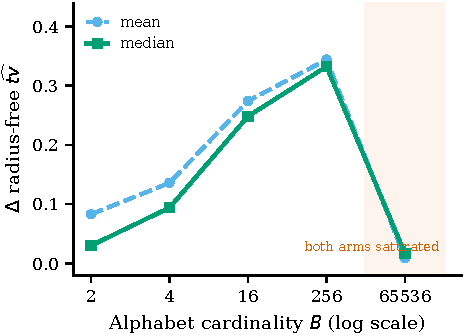
\includegraphics[width=0.52\columnwidth]{figures/paper/fig5_channel_sensitivity.pdf}
\caption{Channel sensitivity. Matched difference in the radius-free estimate
$\widehat{tv}$ between the identifier-dependent and identifier-independent arms
against alphabet cardinality $B$; it grows before both arms saturate. The
quantity is the radius-free estimate only, and no certificate-level implication
follows.}
\label{fig:sensitivity}
\end{figure}

\emph{The full $(M,k)$ grid.} The measured grid behind \Cref{sec:results/horizon} is tabulated in \Cref{tab:grid}.

\begin{table*}[t]
\centering
\small
\caption{The full $(M,k)$ grid, recomputed from the released per-pair ledgers with $m=(2M)^k$ per $M$: pairs clearing the upper-side gate under each bound, and the saturated count ($\widehat{tv}\ge0.99$).}
\label{tab:grid}
\begin{tabular}{r|rrrr|rrrr}
\toprule
& \multicolumn{4}{c|}{clearing Eq.~\eqref{eq:upper}} & \multicolumn{4}{c}{clearing Eq.~\eqref{eq:mfree}} \\
$M$ & $k{=}5$ & $k{=}10$ & $k{=}15$ & $k{=}30$ & $k{=}5$ & $k{=}10$ & $k{=}15$ & $k{=}30$ \\
\midrule
1  & 340 & 28 & 0 & 0 & 363 & 98 & 18 & 0 \\
2  & 47  & 0  & 0 & 0 & 127 & 20 & 4  & 0 \\
4  & 3   & 0  & 0 & 0 & 111 & 10 & 1  & 0 \\
8  & 0   & 0  & 0 & 0 & 94  & 6  & 0  & 0 \\
16 & 0   & 0  & 0 & 0 & 80  & 5  & 0  & 0 \\
\midrule
\multicolumn{9}{l}{\emph{saturated}, $\widehat{tv}\ge0.99$ (of 990 / 990 / 946 / 820)} \\
\midrule
1  & 0   & 6   & 37  & 597 & \multicolumn{4}{c}{(independent of the radius)} \\
2  & 104 & 288 & 545 & 697 & & & & \\
4  & 237 & 587 & 659 & 754 & & & & \\
8  & 333 & 632 & 712 & 784 & & & & \\
16 & 387 & 682 & 764 & 797 & & & & \\
\bottomrule
\end{tabular}
\end{table*}

\subsection{Threshold Sensitivity}
\label{sec:appendix/thresholds}

The gate is a conjunction of an upper and a lower threshold, and the certified
count is driven almost entirely by the upper one. Sweeping each threshold with
the other held at its registered value, on the primary corpus at $k{=}5$,
$M{=}1$, under both lower-side conventions:

\begin{table}[t]
\centering
\small
\caption{Threshold sensitivity at $k{=}5$, $M{=}1$, sweeping each gate threshold with the other held at its registered value, under both lower-side conventions.}
\label{tab:thresholds}
\begin{tabular}{lrr}
\toprule
threshold & full-$n$ & capped \\
\midrule
\multicolumn{3}{l}{\emph{upper threshold}, lower fixed $>0.05$} \\
$<0.30$ & 113 & 112 \\
$<0.40$ & 221 & 220 \\
$<0.50$ & 336 & 335 \\
$<0.60$ & 454 & 453 \\
$<0.70$ & 580 & 579 \\
$<0.80$ & 748 & 747 \\
\midrule
\multicolumn{3}{l}{\emph{lower threshold}, upper fixed $<0.5$} \\
$>0.01$ & 340 & 340 \\
$>0.05$ & 336 & 335 \\
$>0.10$ & 320 & 312 \\
$>0.20$ & 239 & 229 \\
$>0.30$ & 140 & 125 \\
$>0.40$ & 35 & 20 \\
\bottomrule
\end{tabular}
\end{table}

The closed form promised in \Cref{sec:design/frontier} is obtained by solving
\eqref{eq:upper} for the largest $M$ at which $\epshi$ can still fall below the
gate. With equal per-side counts $n$ the surviving margin is
$B(k,n,\alpha) = 0.5 - \widehat{tv} - \sqrt{2\ln(2/\alpha)/n}$, and requiring
$B>0$ turns $m=(2M)^k$ into
\begin{equation}
  M_{\max} \;=\; \Bigl\lfloor \tfrac{1}{2}\bigl(nB^{2}\bigr)^{1/k} \Bigr\rfloor ,
  \label{eq:mmax}
\end{equation}
the largest positive integer satisfying the strict inequality, and $0$ if none
does. This is the same criterion the sweep above evaluates numerically.

The two columns differ only through the lower side's sample cap, and
the full-$n$ column is the paper's convention throughout. Note the asymmetry: on
the upper sweep the cap costs exactly one pair at every rung, while on the lower
sweep it costs nothing until the threshold passes $0.05$ and then costs up to
fifteen, because a stricter lower threshold excludes pairs whose bound the cap
had already lowered.

\subsection{Planning Count and Dependence-Aware Radii}
\label{sec:appendix/track5}

\emph{A planning corollary.} Inverting \eqref{eq:mfree} at equal flow counts
gives the count a pair needs before its interval can close at the gate,
$n > C/(0.5-\widehat{tv})^2$ with $C = 2\ln(2/\alaw) = 8.764$. The constant
enters as $C$, not as $\sqrt{C}$: $\sqrt{C}$ sits inside the radius, so applying
it linearly to the solved form would understate the requirement by $\sqrt{C} \approx 2.96\times$.
Feasibility is a large fraction at coarse resolution and vanishes at fine:
$380$ of $990$ pairs at $k{=}5$, $114$ of $990$ at $k{=}10$, $20$ of $946$ at
$k{=}15$, and none of $820$ at $k{=}30$. Each median must travel with its
feasible fraction, because the conditional distribution is strongly bimodal (at
$k{=}5$ the required count spans $42$ to $2.1\times10^{9}$ with median
$285$), so a bare median would describe a population that does not exist.
The count is a property of a pair's own $\widehat{tv}$, not a budget for the
corpus, and it is reported as a per-pair planning aid rather than a claim.

\emph{Three dependence-aware radii, and why they are not a ranking.} The
upper side's radius assumes i.i.d.\ sampling, so we also measured whether a
radius built for dependence recovers the nominal level at a fixed $n$. At $n{=}60{,}000$, $B{=}64$,
contamination $0.1$ and true $\tv = 0.400$, over $1000$ replicates, a block
bootstrap covers $0.9940$ $[0.9870, 0.9978]$, a cluster-robust sandwich $0.9780$
$[0.9669, 0.9862]$, and a leave-one-block-out Studentized radius $0.9780$
$[0.9669, 0.9862]$. The reading is \emph{not} that one arm works and two fail.
The sandwich takes $z$-multiples of an influence-function standard error and the
leave-one-block-out arm takes $t$-multiples of a jackknife standard error, so the
two are genuinely different constructions, yet they land on the same coverage
count, $978$ of $1000$, with radii $0.033172$ against $0.033117$. That count is
the fact being reported, not the interval agreement that follows from it: a
Clopper--Pearson interval is a function of the successes and $n$ alone, so an
equal count forces an equal interval by construction, and the shared interval is
one number reported twice rather than two independent confirmations. The two code
paths are genuinely distinct: a cluster-robust influence-function variance with
a normal quantile against a leave-one-out jackknife with a $t$ quantile. What
the arms support is therefore a negative: at this nominal level and this replicate
count the two dependence-aware radius forms are indistinguishable, so neither may
be ranked above the other. Judged by the exact two-sided binomial against nominal, the
sandwich and leave-one-block-out coverages are indistinguishable from $0.975$
($978/1000$, $p{=}0.61$) and only the bootstrap deviates ($994/1000$,
$p{<}0.0001$), in the conservative direction. Both readings are reported
because they differ by criterion rather than by result: the Clopper--Pearson
lower endpoint is the \emph{stricter} test, and by it those two arms fall just
below nominal ($0.9669$) while the bootstrap clears it, so an endpoint-based
verdict would call two of three arms failures and a count-based one would not. Two further facts belong with
these numbers. The criterion is one-sided, a replicate is covered when
$\widehat{tv}$ plus its radius reaches the truth, so the i.i.d.\ reference's
design target is $\Phi(r/\mathrm{sd}) = 0.9809$, not the nominal $0.975$; that
$0.0059$ gap is a property of the design, not a coverage failure. A $5000$-replicate check tests whether the signed deviation is
asymmetric, which would be the natural reason for a one-sided radius to differ
from a symmetric one: it is essentially symmetric (skewness $-0.0089$, standard error $0.0346$,
$95\%$ interval $[-0.0768, +0.0590]$, containing zero). A third moment
indistinguishable from zero does not by itself settle whether the interval's
form matters, since those are different functionals: on these draws the two
forms differ by about $11\%$ (both quantiles taken on the mean-centred
deviation), so they are not interchangeable, against a normal-theory gap
of $12.6\%$. Whether that difference changes
a \emph{coverage} verdict is a separate question, and one we did not test: these
are quantiles of the realised $D$ array, which establish that the forms differ,
not that a computable per-replicate one-sided radius closes any gap. \textbf{What these arms validate is a modelled block law only.}
They are synthetic block-law draws at one block size and one divergence; we did
not test coverage on real traffic, and nothing here says coverage holds on the
corpus.

\subsection{Compute Resources}
\label{sec:appendix/compute}

Per-step timings and per-detector device assignments. The independent-corpus
bracket ran in about 21 minutes on eight CPU workers, the channel-sensitivity
sweep in about 31 minutes, and the known-truth estimator control reuses a
cached occupancy table and finishes in under a minute. LightGBM and the
prototype rejector executed on CPU; RoNeTC ran on a single consumer-grade GPU.
No result here depends on a large-scale cluster.

\begin{table*}[t]
\centering
\small
\caption{Upper-side coverage calibration (seed 20260917), $200$ replicates per cell. Both arms share one generator, $Q=(1-\delta)P+\delta\,\mathbb{1}_{0}$ over a $32$-symbol alphabet, and the same reported radius; the i.i.d.\ column is the control and the $B$ columns inject within-service dependence (contamination $0.1$). Entries are covered replicates out of $200$ with the two-sided $95\%$ Clopper--Pearson lower endpoint in parentheses, and the criterion is whether that endpoint falls below the nominal $0.975$. Triviality depends on $(\mathrm{TV}, n)$ alone: both arms use one radius, and a cell is trivial when that radius reaches the true distance ($\mathrm{TV}/\mathrm{radius}\le 1$), so every column of a trivially-guaranteed cell is marked `--': there coverage is certain, not measured. Every cell that is neither trivial nor one of the two $(\mathrm{TV},n)=(0.40,50953)$ and $(0.40,107065)$ cells is identical, $200/200$ with lower endpoint $0.9817$ in all four columns; those two rows differ from $200/200$ only in their $B{=}64$ column, which carries the confirmation loss of \Cref{sec:discussion/limitations}. The $15$ folded cells are the $20$ rows minus the $3$ trivially-guaranteed rows and the $2$ breach rows, namely $\mathrm{TV}=0.05$ at $n\ge 50953$; $\mathrm{TV}\in\{0.10,0.20,0.30,0.40\}$ at $n=10988$; $\mathrm{TV}\in\{0.10,0.20,0.30\}$ at $n\in\{50953,107065\}$; and $\mathrm{TV}\in\{0.20,0.30,0.40\}$ at $n=2791$. Each is $200/200$ with lower endpoint $0.9817$ in all four columns.}
\label{tab:coverage}
\begin{tabular}{rrrrrr}
\toprule
$\mathrm{TV}$ & $n$ & i.i.d. & $B{=}1$ & $B{=}8$ & $B{=}64$ \\
\midrule
0.05 & 2791 & -- & -- & -- & -- \\
0.05 & 10988 & -- & -- & -- & -- \\
0.10 & 2791 & -- & -- & -- & -- \\
\midrule
\multicolumn{2}{l}{15 further cells (see caption)} & 200/200 (0.9817) & 200/200 (0.9817) & 200/200 (0.9817) & 200/200 (0.9817) \\
\midrule
0.40 & 50953 & 200/200 (0.9817) & 200/200 (0.9817) & 200/200 (0.9817) & 199/200 (0.9725) \\
0.40 & 107065 & 200/200 (0.9817) & 200/200 (0.9817) & 200/200 (0.9817) & 196/200 (0.9496) \\
\bottomrule
\end{tabular}
\end{table*}

\emph{The LP-weighted floor.} The comparison floor quoted in
\Cref{sec:design/problem} comes from a linear program over the same $990$-pair
input. Its variables are non-negative weights $w_{ij}\ge 0$ on ordered pairs;
the constraint is that every class's total weight be uniform,
$\sum_{j\ne i}(w_{ij}+w_{ji})=1$ for each of the $K$ known classes and $0$ for
the unknown class. Grouping by $i$ gives
$\sum_{i\ne j}w_{ij}(\mathrm{err}_i+\mathrm{err}_j)=\sum_i \mathrm{err}_i$ over the
$K$ known classes, since the constraint is that inner sum for each of them. That
left side is therefore the known-class error total, so
$\sum_{i\ne j}w_{ij}(\mathrm{err}_i+\mathrm{err}_j)\le M\,\mathbb{E}[\mathrm{err}]$
with the expectation over all $M$ classes, the unknown term entering as zero,
and strict by $K/M$ if it is averaged over the known classes alone. The objective is
$\max\sum_{i\ne j}w_{ij}(1-\epsilon_{\mathrm{hi},ij})$, every term of
which is a certified upper bound. The weights range over the $K$ known classes
only, the unknown-class terms being discarded as before, while the denominator
keeps $M = K+1$, so the open-set discarded-term property is preserved as well. The
maximum over feasible weights is valid a fortiori: each weight is non-negative
and each $1-\epsilon_{\mathrm{hi},ij}$ is no larger than the $1-\tv_{ij}$ it stands for,
so the objective can only undershoot the true value. The uniform point under
\emph{this} constraint is $w_{ij}=1/[2(K-1)]$, whose row sum $2(K-1)w$ is exactly
$1$, and it recovers the uniform floor $0.197$ of \eqref{eq:floor} up to the
ratio $(M-1)/(K-1)$ between the two normalisations: $(M-1)/(K-1)=45/44$ here, so
the two differ by about $2\%$ and neither is a feasible point of the other's
problem. We quote each floor against the constraint that defines it rather than
treating them as one point. We report the LP floor as a comparison rather than a
headline for the reasons given in \Cref{sec:design/problem}.


\subsection{Detector Validation Table}

The nine-cell containment test behind \Cref{sec:results/detector_validation} is tabulated in \Cref{tab:detectors}.

\begin{table}[t]
\centering
\caption{Detector validation on the informative stratum ($\epshi < 0.5$, 340 pairs). Each cell is a one-sided binomial test of floor violations against a pre-registered null rate $\ptest = 0.05$, that rate being the tolerable violation share rather than the certified floor; none rejects the null, so no detector's violation share is shown to exceed it, and failing to reject is not evidence that the floor is tight. The fourth intended detector is \emph{not\_run}: it contributes no information and is not counted as a pass.}
\label{tab:detectors}
\begin{tabular}{lrrrr}
\toprule
Detector & holdout & viol. & rate & $p$ \\
\midrule
LightGBM & 0.05 & 8 & 0.0235 & 0.9954 \\
 & 0.1 & 8 & 0.0235 & 0.9954 \\
 & 0.2 & 10 & 0.0294 & 0.9765 \\
\midrule
Prototype & 0.05 & 3 & 0.0088 & 1.0000 \\
 & 0.1 & 4 & 0.0118 & 1.0000 \\
 & 0.2 & 4 & 0.0118 & 1.0000 \\
\midrule
RoNeTC & 0.05 & 3 & 0.0088 & 1.0000 \\
 & 0.1 & 3 & 0.0088 & 1.0000 \\
 & 0.2 & 2 & 0.0059 & 1.0000 \\
\bottomrule
\end{tabular}
\end{table}

% The reference list is set one step smaller and without inter-item padding:
% USENIX counts references outside the 13-page body, but the camera-ready cap of
% 20 total pages is a hard bound and the list otherwise spills one page.
% No content is dropped. The size/sep changes are applied through natbib's own
% bibliography hooks rather than by wrapping \bibliography in a group, which
% suppresses the \bibdata line in the .aux and leaves bibtex with nothing to do.
\makeatletter
\renewcommand{\bibfont}{\footnotesize}
\setlength{\bibsep}{1.2pt plus 0.2ex}
\makeatother



\bibliographystyle{plainnat}
\bibliography{references}

\end{document}
